% !TEX encoding = UTF-8 Unicode
% !TEX TS-program = XeLaTeX
% !BIB TS-program = biber
% !TEX useTabsWithFiles
% !TEX tabbedFile{TitlePage.tex}
% !TEX tabbedFile{Introduction.tex}
% !TEX tabbedFile{DeployingAndUsing.tex}
% !TEX tabbedFile{Building.tex}
% !TEX tabbedFile{Appendices.tex}
% !TEX tabbedFile{acronyms.tex}

\documentclass[12pt,letterpaper,openany,oneside,draft]{book}

%\usepackage{xifthen}
%\newboolean{enablePortionMarkings}
%\setboolean{enablePortionMarkings}{true}

\usepackage{parskip}				% Begin paragraphs with empty line, not indent
\usepackage{xcolor}
\usepackage{fancyvrb}
\usepackage{titling}
\usepackage{fnpct}
\usepackage[inline]{enumitem}
\usepackage{acro}
\usepackage[final]{graphicx}
\usepackage{booktabs}
\usepackage{array}
\usepackage{ragged2e}
%\usepackage{colortbl}
%\usepackage{rotating}
%\usepackage{marginnote}
\usepackage{relsize}
\usepackage{fancyhdr}
%\usepackage{lastpage}
%\usepackage{lipsum}
\usepackage{amsmath}
\usepackage{amssymb}
%\usepackage[retainorgcmds]{IEEEtrantools}
%\usepackage{skmath}
%\usepackage{tikz}
\usepackage{path}
\usepackage{dirtree}
%\usepackage[firstpage]{draftwatermark}
%\usepackage{todonotes}
%\usepackage[T1]{fontenc}		% Enables curly braces in emails within \institute
\usepackage[style=numeric,backref,backend=biber]{biblatex}
\usepackage{fontspec,xltxtra,xunicode,unicode-math,iffont}
\usepackage[unicode,final]{hyperref}	% Should be the last use-package command
\def\UrlBreaks{\do\/\do-}

%\newcommand{\red}[1]{{\color{red}#1}}
%\newcommand{\paraleader}[1]{\textbf{#1}}
\newcommand{\urlcite}[1]{\footnote{\url{#1}}}
\newcommand{\headingrule}{\midrule[\heavyrulewidth]}
%\newcommand{\themestatement}[1]{\framebox{\parbox{0.97\columnwidth}{\emph{#1}}}}
\newcommand{\githubOrg}{raytheonbbn}
\newcommand{\boostversion}[1]{1{#1}84{#1}0}
\newcommand{\lmdbversion}{0.9.31}

% !TEX encoding = UTF-8 Unicode
% !TEX TS-program = XeLaTeX

\DeclareAcronym{bbn}{
	short					=BBN,
	long					=RTX BBN Technologies,
	short-plural		='s,
	long-plural			=',
}
\DeclareAcronym{cdt}{
	short					=CDT,
	long					=Eclipse C/C++ Developers Toolkit,
	extra					={A set of Eclipse plug-ins to facilitate C and C++ development in that environment.},
}
\DeclareAcronym{daml}{
	short					=DAML,
	long					=DARPA Agent Markup Language,
}
\DeclareAcronym{darpa}{
	short					=DARPA,
	long					=Defense Advanced Research Projects Agency,
	short-plural		='s,
	long-plural			='s,
}
\DeclareAcronym{dll}{
	short					=DLL,
	long					=Dynamic Link Library,
	extra					={Often used synonymously with ``shared library'' or ``shared object.''},
}
\DeclareAcronym{http}{
	short					=HTTP,
	long					=HyperText Transfer Protocol,
}
\DeclareAcronym{ide}{
	short					=IDE,
	long					=Integrated Development Environment,
}
\DeclareAcronym{jni}{
	short					=JNI,
	long					=Java Native Interface,
	extra					={A facility within the Java platform to allow Java code to directly call native code.},
}
\DeclareAcronym{jvm}{
	short					=JVM,
	long					=Java Virtual Machine,
}
\DeclareAcronym{kb}{
	short					=KB,
	long					=Knowledge Base,
}
\DeclareAcronym{lmdb}{
	short					=LMDB,
	long					=Lightning Memory-Mapped Database Manager,
}
\DeclareAcronym{nas}{
	short					=NAS,
	long					=Network-Attached Storage,
}
\DeclareAcronym{owl}{
	short					=OWL,
	long					=Web Ontology Language,
	short-indefinite	=an,
	long-indefinite	=a,
}
\DeclareAcronym{pmnt}{
	short					=Parliament,
	long					=Parliament™,
	short-plural		='s,
	long-plural			='s,
	extra					={BBN's triple store, so named because ``parliament'' is the collective noun for a group of owls.  A triple store is a specialized database tuned to the unique needs of the Semantic Web data representation.},
	pdfstring			=Parliament/'s,
}
\DeclareAcronym{raid}{
	short					=RAID,
	long					=Redundant Array of Inexpensive Disks,
}
\DeclareAcronym{rdf}{
	short					=RDF,
	long					=Resource Description Framework,
}
\DeclareAcronym{rdfs}{
	short					=RDFS,
	long					=RDF Schema,
}
\DeclareAcronym{san}{
	short					=SAN,
	long					=Storage Area Network,
}
\DeclareAcronym{sparql}{
	short					=SPARQL,
	long					=SPARQL Protocol and RDF Query Language,
	extra					={If this seems confusing, it is because SPARQL is a recursive acronym.},
}
\DeclareAcronym{swrl}{
	short					=SWRL,
	long					=Semantic Web Rule Language,
}
\DeclareAcronym{url}{
	short					=URL,
	long					=Uniform Resource Locator,
	extra					={The address of a page on the World Wide Web, typically starting with the prefix ``http:'' or ``https:''.},
}
\DeclareAcronym{w3c}{
	short					=W3C,
	long					=World Wide Web Consortium,
}

\bibliography{references}

\title{\acl{pmnt} User Guide}
\author{Ian Emmons}
\date{\today}
%\setlength{\droptitle}{-50pt}
%\pretitle{\begin{center}\LARGE}
%\posttitle{\par\end{center}\vskip 0.5em}
%\preauthor{\begin{center}\large\lineskip 0.5em\begin{tabular}[t]{c}}
%\postauthor{\end{tabular}\par\end{center}}
%\predate{\begin{center}\large}
%\postdate{\par\end{center}}

\settofirstfound{\mainfont}{Georgia,TeX Gyre Bonum}
\settofirstfound{\sansfont}{Verdana,TeX Gyre Heros}
\settofirstfound{\monofont}{Menlo,Andale Mono,Lucida Console,Courier New}
\settofirstfound{\mathfont}{TeX Gyre Bonum Math,STIX Math}
\defaultfontfeatures{Mapping=tex-text}
\setmathfont{\mathfont}
\setmainfont{\mainfont}
\setsansfont{\sansfont}[Scale=MatchLowercase]
\setmonofont{\monofont}[Scale=MatchLowercase,PunctuationSpace=WordSpace,Mapping=]

\fvset{tabsize=3}

\pagestyle{fancy}
\renewcommand{\chaptermark}[1]
	{\markboth{\chaptername \ \thechapter.\ #1}{}}
\fancyhead[L]{\textsl{\leftmark}}
\fancyhead[R]{}
\setlength{\headheight}{15pt}

%\urlstyle{rm}
\definecolor{hyperlinkcolor}{rgb}{0,0,0.625}
\hypersetup{
	final=true,
	unicode=true,
	bookmarksnumbered=true,
	pdftitle={Parliament User Guide},
	pdfauthor={\theauthor},
	colorlinks=true,
	allcolors=hyperlinkcolor
}

%\SetWatermarkAngle{45}
%\SetWatermarkLightness{0.8}		% 1 = white, 0 = black
%\SetWatermarkFontSize{5cm}
%\SetWatermarkScale{1.2}
%\SetWatermarkText{\textsc{Draft}}

\hyphenation{Arc-GIS Arc-Map}
\hyphenation{co-ref-er-ence co-ref-er-enc-es}
\hyphenation{da-ta-base da-ta-bas-es}
\hyphenation{geo-spa-tial}
\hyphenation{ra-pid-ly}
\hyphenation{ray-the-on}
\hyphenation{serv-let serv-lets}
\hyphenation{trac-ta-ble}
\hyphenation{war-fight-er war-fight-ers}

\fvset{tabsize=3}

\begin{document}
\acuse{pmnt} % Only long & short forms, never "first appearance"
\acuse{url} % This one is too common to bother spelling it out

\frontmatter
% !TEX encoding = UTF-8 Unicode
% !TEX TS-program = XeLaTeX
% !TEX root = ParliamentUserGuide.tex

\begin{titlepage}
	\centering

	\vspace*{\baselineskip}

	\rule{\textwidth}{1.6pt}\vspace*{-\baselineskip}\vspace*{2pt}
	\rule{\textwidth}{0.4pt}

	\vspace{0.75\baselineskip}

	{\LARGE\acl{pmnt}\\User Guide\\}

	\vspace{0.75\baselineskip}

	\rule{\textwidth}{0.4pt}\vspace*{-\baselineskip}\vspace{3.2pt}
	\rule{\textwidth}{1.6pt}

	\vspace{2\baselineskip}

	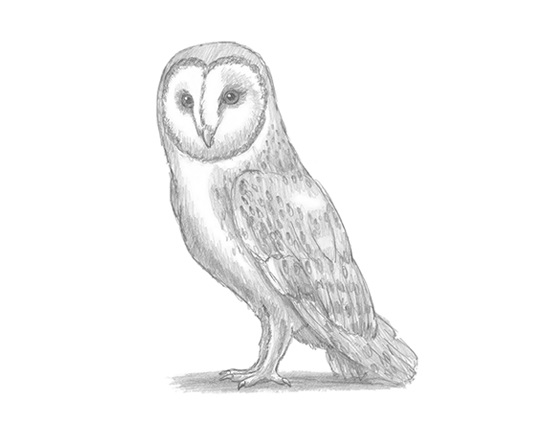
\includegraphics[width=0.3\textwidth]{includes/BarnOwl.jpeg}

	\vspace*{4\baselineskip}

	{\Large\theauthor\\}

	\vspace{0.5\baselineskip}

	\textit{\thedate}

	\vfill

	\textit{Copyright © 2001-2021,\\
	\acl{bbn}, Inc.\\
	All rights reserved.}

	{\small Fonts used:  \emph{\mainfont, \sansfont, \monofont,} and \emph{\mathfont}}
\end{titlepage}
\tableofcontents
\listoffigures
\listoftables

\mainmatter

% !TEX encoding = UTF-8 Unicode
% !TEX TS-program = XeLaTeX
% !TEX root = ParliamentUserGuide.tex

%%%%%%%%%%%%%%%%%%%%%%%%%%%%%%%%%%%%%%%%%%%%%%%%%%
\chapter{Introduction to \acl{pmnt}}

\acl{pmnt} is a high-performance semantic graph store (also called a triple store) and reasoner designed for the Semantic Web\urlcite{http://www.w3.org/2001/sw/}.  \acf{bbn} developed \ac{pmnt} initially under the name DAML DB\urlcite{http://www.daml.org/2001/09/damldb/} under \acp{darpa} \ac{daml} program. \ac{bbn} later extended \ac{pmnt} for internal use in its R\&D programs and released \ac{pmnt} as an open source project under the BSD license\urlcite{http://opensource.org/licenses/bsd-license.php} on SemWebCentral\urlcite{http://parliament.semwebcentral.org/} in 2009.  In 2018, \ac{bbn} migrated the \ac{pmnt} open source project to GitHub\urlcite{https://github.com/\githubOrg/parliament} under the same license.

\acl{pmnt} is a trademark of \acl{bbn}.  It is so named because a group of owls is properly called a \emph{parliament} of owls.

%%%%%%%%%%%%%%%%%%%%%%%%%%%%%%%%%%%%%%%%%%%%%%%%%%
\section{Background}

The Semantic Web employs a different data model than a relational database.  A relational database stores data in tables (rows and columns) while \ac{rdf}\urlcite{http://www.w3.org/RDF/} represents data as a directed graph of ordered triples of the form (subject, predicate, object).  Accordingly, a Semantic Web data store is often called a semantic graph, triple store, knowledge base, or graph store.

A relational database can store a directed graph, and some graph stores are in fact implemented as a thin interface layer wrapping a relational database.  However, the query performance of such implementations is usually poor.  This is because the only straightforward way to store the graph with the required level of generality is to use a single table to store all the triples, and this schema tends to defeat relational query optimizers.

Early in the Semantic Web's evolution, \ac{bbn} encountered exactly this problem, and so the graph store we now call \ac{pmnt} was born.  The goal of \ac{pmnt} was to create a storage mechanism optimized specifically to the needs of the Semantic Web, and the result was a dramatic speed boost for \acp{bbn} Semantic Web programs.  Since its initial conception, \ac{pmnt} has served as a core component of several projects at \ac{bbn} for a number of U.S.\ Government customers.

%%%%%%%%%%%%%%%%%%%%%%%%%%%%%%%%%%%%%%%%%%%%%%%%%%
\section{\ac{pmnt} Architecture}

\ac{pmnt} combines customized versions of the Web interface and query processor of Jena\urlcite{https://jena.apache.org/} with a high-performance storage engine and an innovative storage layout to deliver a complete triple store solution that is compatible with the  \ac{rdf}, \ac{owl}\urlcite{http://www.w3.org/2007/OWL/}, and \ac{sparql}\urlcite{http://www.w3.org/2009/sparql/wiki/Main\_Page} standards from the \ac{w3c} \autocite{KoEmDe:09:ParliamentIndexing}.

In addition, \ac{pmnt} includes a high-performance rule engine, which applies a set of inference rules to the directed graph of data in order to derive new facts.  This enables \ac{pmnt} to automatically and transparently infer additional facts and relationships in the data to enrich query results.  \acp{pmnt} rule engine currently implements all of the inference rules of \ac{rdfs} plus selected elements of \ac{owl} RL.

Figure~\ref{figure-parliament-layers} depicts the layered architecture of \ac{pmnt}.  The storage layer of \ac{pmnt} is written in C++, while the remainder is Java code.  Integrated with the Jena query processor are a number of useful extras, such as support for named graphs, accelerated reification support, and temporal, geospatial, and numerical indexes \autocites{Ko:2010}{BaKo:2012}.

\begin{figure}[htbp]
	\centering
	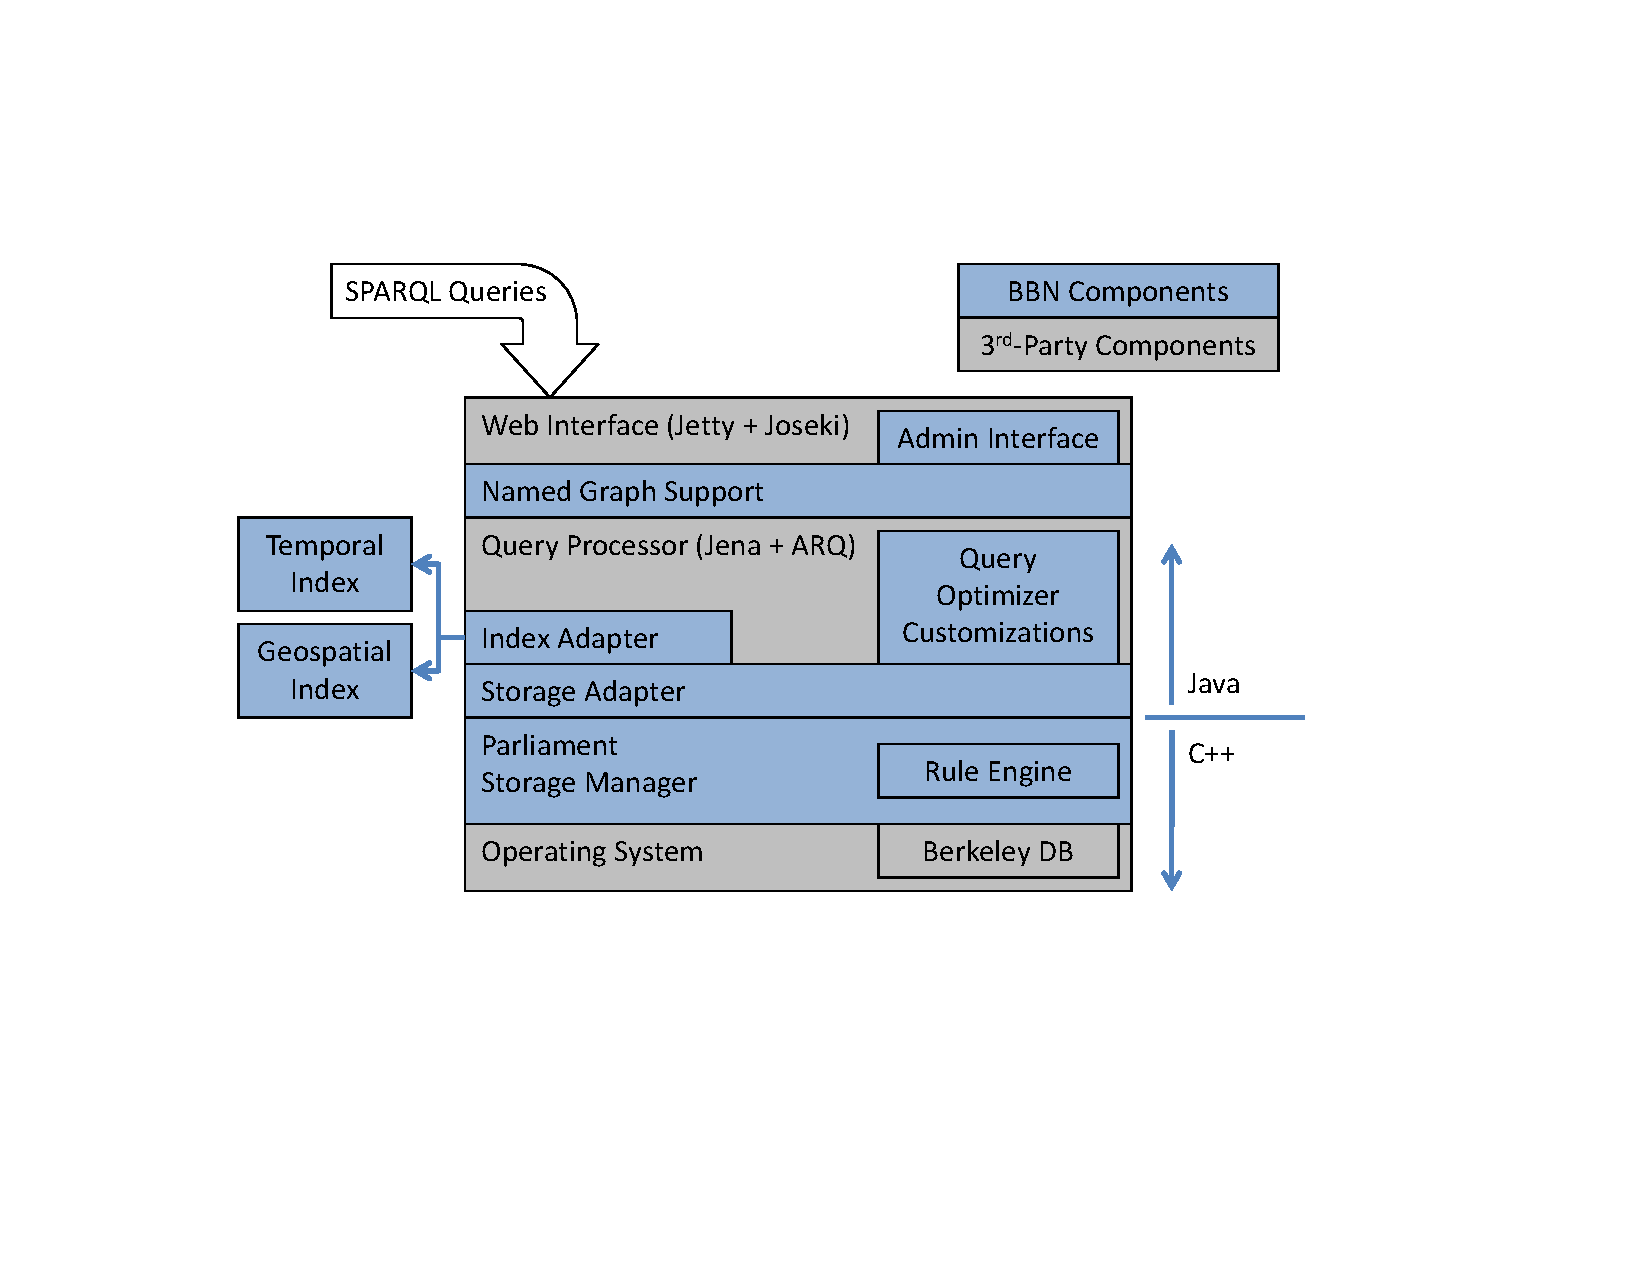
\includegraphics[width=1.0\textwidth]{includes/architecture.pdf}
	\caption{Layered \ac{pmnt} Architecture}
	\label{figure-parliament-layers}
\end{figure}

% !TEX encoding = UTF-8 Unicode
% !TEX TS-program = XeLaTeX
% !TEX root = ParliamentUserGuide.tex

%%%%%%%%%%%%%%%%%%%%%%%%%%%%%%%%%%%%%%%%%%%%%%%%%%
\chapter{Deploying and Using \acl{pmnt}}
\label{chapter-deploying-and-using}

There are several ways to use \ac{pmnt}.  By far the most common is as a server application that exposes a \ac{sparql} endpoint.  \acp{pmnt} Docker image and its more traditional binary distribution directly support this usage, running \ac{pmnt} within the included Jetty servlet engine.  See Sections~\ref{section-std-container-deploy} and~\ref{section-std-server-deploy} for instructions.

\ac{pmnt} can also be used with other servlet engines such as Tomcat and Glassfish (see Section~\ref{section-parliament-with-jena-and-tomcat}) or as an in-process library (Section~\ref{section-parliament-in-process}).

Pre-built binaries for common platforms are available on the \ac{pmnt} Web site\urlcite{https://github.com/SemWebCentral/parliament/releases}.  You can also build \ac{pmnt} yourself (see Chapter~\ref{chapter-building-parliament}).

This chapter starts with instructions for running a \ac{pmnt} container (Section~\ref{section-std-container-deploy}) and for installing a \ac{pmnt} server (Section~\ref{section-std-server-deploy}), followed by a discussion of the \ac{pmnt} configuration file (Section~\ref{section-configuring-pmnt}).  Then comes a detailed discussion of each of the less common deployment scenarios.  The chapter concludes with a discussion of \acp{pmnt} utilities and some troubleshooting hints (Sections~\ref{section-parliamentadmin-utility} and~\ref{section-troubleshooting}, respectively).

%%%%%%%%%%%%%%%%%%%%%%%%%%%%%%%%%%%%%%%%%%%%%%%%%%
\section{Deploying a \ac{pmnt} Container}
\label{section-std-container-deploy}

\acp{pmnt} Docker image can be found on Docker Hub here:
\begin{quote}
\texttt{idemmons/parliament:«version»}
\end{quote}

To run the container, use this command (with line breaks added for readability):
{\small
\begin{verbatim}
docker run -d -p 80:8089 --name=parliament-«version»
   --mount type=volume,src=parliament-data,dst=/var/parliament-data
   --env PARLIAMENT_JAVA_HEAP_SIZE=512m
   --env PARLIAMENT_BDB_CACHE_SIZE=512m,1
   idemmons/parliament:«version»
\end{verbatim}
}

As given here, the mount option will create a local Docker volume called \path|parliament-data| to contain \acp{pmnt} data files and logs.  Using variations of this option, you can cause the container to store the data files and logs in a broad variety of locations and file systems, such as on an external storage array.  (See the Docker documentation for more information.)

Alternately, Docker can store \acp{pmnt} data files and logs in a local directory on the container's host with this syntax:
{\small
\begin{verbatim}
docker run -d -p 80:8089 --name=parliament-«version»
   --mount type=bind,src=/host/directory,dst=/var/parliament-data
   --env PARLIAMENT_JAVA_HEAP_SIZE=512m
   --env PARLIAMENT_BDB_CACHE_SIZE=512m,1
   idemmons/parliament:«version»
\end{verbatim}
}

The two environment variables are optional.  If they are left out, the default values used will be the values shown in the command line above.  (See Sections~\ref{section-pmnt-startup-script} and~\ref{section-main-config} for discussions of these settings.)  Table~\ref{table-pmnt-container-connect-urls} lists the endpoints exposed by the running container, as discussed in Section~\ref{section-std-server-usage}.

\begin{table}[htbp]
	\centering
	\begin{tabular}{ll}
		\acs*{http} interface: & \nolinkurl{http://«host»/parliament}\\
		\ac{sparql} endpoint: & \nolinkurl{http://«host»/parliament/sparql}\\
		Bulk loader: & \nolinkurl{http://«host»/parliament/bulk}\\
	\end{tabular}
	\caption{\acs*{pmnt} Container Connection \acsp*{url}}
	\label{table-pmnt-container-connect-urls}
\end{table}



%%%%%%%%%%%%%%%%%%%%%%%%%%%%%%%%%%%%%%%%%%%%%%%%%%
\section{Deploying a \ac{pmnt} Server}
\label{section-std-server-deploy}

A \ac{pmnt} distribution is a compressed archive containing a ready-to-run \ac{pmnt} server, with the following naming convention:
\begin{quote}
	\texttt{parliament-\textbf{\textit{x.y.z}}-\textbf{\textit{platform}}.zip}
\end{quote}
Here \texttt{\textbf{\textit{x.y.z}}} is the \ac{pmnt} version number and \texttt{\textbf{\textit{platform}}} indicates the platform, as shown in Table~\ref{tbl:SupportedPlatforms}\footnote{At present, only Intel/AMD architectures are supported.  We expect to support Apple Silicon and ARM binaries in a future release.}.
\begin{table}[htbp]
	\centering
	\begin{tabular}{lll}
		\toprule
		\emph{Platform}	& \emph{Description}				& \emph{Binaries}\\
		\headingrule
		\path|mac|			& Mac OS Catalina and newer	& 64-bit\\
		\path|rhel8|		& Red Hat Enterprise Linux 8	& 64-bit\\
		\path|ubuntu20|	& Ubuntu Linux 20, LTS			& 64-bit\\
		\path|win-64|		& Windows 10 and newer			& 64-bit\\
		\path|win-32|		& Windows 10 and newer			& 32-bit\\
		\bottomrule
	\end{tabular}
	\caption{Supported Platforms}
	\label{tbl:SupportedPlatforms}
\end{table}
If you are building \ac{pmnt} yourself according to the instructions in Chapter~\ref{chapter-building-parliament}, then these archives appear in the \path|target/distro| directory at the end of the build process.

As shown in Table~\ref{tbl:SupportedPlatforms}, on Windows there is a choice between 32-bit and 64-bit builds.  Whenever possible, use the 64-bit version, because 32-bit \ac{pmnt} is limited to 5--10 million statements.

\subsection{Installing for the First Time}
\label{section-std-server-init-deploy}

Once you have downloaded a distribution, these steps will yield a functioning \ac{kb}:
\begin{enumerate}
	\item Extract the archive to your preferred location.  On UNIX-like systems, \path|/usr/opt/ParliamentKB| or \path|/usr/local/ParliamentKB| is a likely choice.  On Windows, \path|C:\Program Files\ParliamentKB| is customary.  The instructions that follow refer to this directory as simply \path|ParliamentKB|.

	\item On Windows, install the C and C++ run-time libraries.  You can find installers for these in the following directory:
	\begin{quote}
		\path|ParliamentKB/RedistributablePackages|
	\end{quote}

	\item On Windows, open a PowerShell, switch to the \path|ParliamentKB| directory, and invoke the startup script to start the \ac{pmnt} server:
	\begin{quote}
		\path|.\parliament.ps1 -foreground|
	\end{quote}
	For backwards compatibility, you may also use a command prompt and type:
	\begin{quote}
		\path|StartParliament.bat|
	\end{quote}

	On other platforms, open a shell, switch to the \path|ParliamentKB| directory, and start \ac{pmnt} using this command:
	\begin{quote}
		\texttt{./parliament foreground}
	\end{quote}
	For backwards compatibility, you an also type:
	\begin{quote}
		\texttt{./StartParliament.sh}
	\end{quote}

	Whatever platform you are using, this starts \ac{pmnt} as a command line process running under the current terminal.  You can shut down the server by typing ``exit'' or ``Ctrl+C''.
\end{enumerate}

The procedure above directly starts the \acp{pmnt} server.  However, in many cases it is preferable to run \ac{pmnt} as a Windows service or as a Linux/UNIX daemon.

\subsubsection{Installing as a Windows Service}

Use the following procedure to install \ac{pmnt} as a Windows service.

If you want \ac{pmnt} to run under a dedicated account, start by creating that account.  This step is optional.

Next create a data directory in a location of your choice.  One reasonable option is \path|C:\ProgramData\parliament-data|.  \ac{pmnt} will store its content here, as well as logging and temporary files.  Ensure that this directory is writable by the user established above.  (Even if you did not create such a user, you may need to grant access to the ``Local Service'' account.)

Now unzip the \ac{pmnt} distribution to a location of your choice, such as \path|C:\Program Files\ParliamentKB|.  It is fine for this directory to be read-only for the user established above.

It is important to note that neither of the two locations above should be on a mapped network drive.  This is because the mapping is an artifact of your user login, and services run outside that context.

Make the following configuration changes:

\begin{itemize}
	\item In \path|parliament.ps1|, uncomment the two lines for the user name and password and fill in the user name and password established above, if you created one.  If not, skip this step.

	\item Also in \path|parliament.ps1|, you may wish to edit certain other parameters, such as the host and port or the memory allocated to the JVM (see Section~\ref{section-configuring-pmnt}).  This step is also optional.

	\item In \path|ParliamentKbConfig.txt|, set the \path|kbDirectoryPath| entry to the absolute path of the data directory you created above.
\end{itemize}

Finally, from the \ac{pmnt} directory, issue this command in PowerShell:

\begin{verbatim}
     .\parliament.ps1 -install
\end{verbatim}

Then open the Services management console, select \ac{pmnt}, and click the start button.

At this point, \ac{pmnt} is running in the background, and whenever the system is shut down and restarted, \ac{pmnt} will also properly shut down and restart.  You can monitor and control (start, stop, and restart) \ac{pmnt} via the Services management console as above.

To uninstall \ac{pmnt} as a Windows service, shut it down and then run this command:
\begin{verbatim}
     .\parliament.ps1 -uninstall
\end{verbatim}

If you change any of the parameters in \path|parliament.ps1| after installing as a service, (see Section~\ref{section-configuring-pmnt}) or upgrade your Java installation, you will need to uninstall and re-install the service in order to have those changes reflected in the installed service definition.

\subsubsection{Installing as a Linux Daemon}

This section is focused on variants of Linux that support systemd, such as RHEL and Ubuntu.  For setup on non-systemd Linux, please use the next section.

To install \ac{pmnt} as a systemd service, we begin by establishing a system account (and group) under which \ac{pmnt} will run.  To do this from scratch, use the following command:

\begin{quote}
	\texttt{sudo adduser --system --group parliament}\hfill (Ubuntu)
	\texttt{sudo useradd --system -U parliament}\hfill (RHEL)
\end{quote}

Next we need to create a data directory in a location of your choice, such as \path|/var/parliament-data|.  \ac{pmnt} will store its content here, as well as logging and temporary files.  Ensure that this directory is owned and writable by the group and user established above:

\begin{verbatim}
     sudo chmod u=rwx,go=rx /var/parliament-data
     sudo chown -R parliament:parliament /var/parliament-data
\end{verbatim}

Now unzip the \ac{pmnt} distribution to a location of your choice, such as \path|/opt/ParliamentKB| or \path|/usr/local/ParliamentKB|.  It is fine for this directory to be owned by root and read-only for the group and user established above.

Make the following configuration changes:

\begin{itemize}
	\item In \path|parliament|, uncomment the line containing \path|DAEMON_USER| and set it to the name of the user created above.

	\item Also in \path|parliament|, you may wish to edit certain other parameters, such as the host and port or the memory allocated to the JVM (see Section~\ref{section-configuring-pmnt}).  This step is optional.

	\item In \path|ParliamentKbConfig.txt|, set the \path|kbDirectoryPath| entry to the absolute path of the data directory you created above.
\end{itemize}

Finally, from the \ac{pmnt} directory, issue these commands:

\begin{verbatim}
     sudo ./parliament install
     sudo systemctl start parliament
\end{verbatim}

At this point, \ac{pmnt} is running in the background, and whenever the system is shut down and restarted, \ac{pmnt} will also properly shut down and restart.  You control \ac{pmnt} via the \path|systemctl| command:
\begin{quote}
	\texttt{sudo systemctl \{ start | stop | restart \} parliament}
\end{quote}

You can check whether \ac{pmnt} is running with either of these commands:

\begin{verbatim}
     ps -ef | grep -i parliament | grep -v grep
     sudo systemctl show parliament
\end{verbatim}

To uninstall \ac{pmnt} as a systemd service, run this command:
\begin{verbatim}
     sudo ./parliament uninstall
\end{verbatim}

\subsubsection{Installing as a UNIX Daemon}

For UNIX and non-systemd Linux variants, this command will run \ac{pmnt} as a detached process suitable to run as a daemon:

\begin{quote}
	\texttt{./parliament \{ start | stop | restart \}}
\end{quote}

However, there is currently no built-in support for wiring this into the operating system's infrastructure for starting and stopping daemon processes, because this infrastructure varies from platform to platform.  In the future, this may be remedied for specific platforms, such as MacOS X.



\subsection{Upgrading an Existing Installation}
\label{section-std-server-upgrade}

When upgrading an existing \ac{pmnt} installation to a newer version, the procedures of Section~\ref{section-std-server-init-deploy} are generally not sufficient because they ignore the migration of the data.  The \ac{pmnt} development team strives to maintain compatibility of file formats whenever possible.  In such cases, all that is required is to move the \path|kb-data| subdirectory of your \ac{pmnt} installation into the new \ac{pmnt} installation.  Of course, if you have customized \acp{pmnt} configuration, you will also need to make those changes in the new installation as well.

However, from time to time \acp{pmnt} file formats do change, and in such cases a different migration procedure is required.  Following this procedure even in those cases where it is not required has some benefits as well, since it frees up any unused space in the \ac{pmnt} data files.  This is the way to perform such a migration:

\begin{enumerate}
	\item\label{upgrade-procedure-first-step}\textbf{\emph{Before upgrading,}} point your browser at your \ac{pmnt} server.  The \ac{url} for this is \nolinkurl{http://<host>:<port>/parliament/}.  By default this will be \nolinkurl{http://localhost:8089/parliament/}.

	\item Click on the ``Export'' link.

	\item\label{item-export-download}Click on the ``Export Repository'' button.  This will start a download whose file name looks like this:
\begin{quote}\path|parliament-export-localhost-<date>-<time>.zip|\end{quote}

	\item When the download finishes, shut down \ac{pmnt}.  Rename the \ac{pmnt} installation directory if you want your upgraded installation to reside in the same place.

	\item Unzip the new version of \ac{pmnt} to your desired location, customize the new installation's settings as required (see Section~\ref{section-configuring-pmnt}), and start up the new \ac{pmnt} installation.

	\item Point your browser at the new \ac{pmnt} server.  The \ac{url} is the same as the one in Step~\ref{upgrade-procedure-first-step} above.

	\item Click on the ``Insert Data'' link.  In the ``Import Repository'' section, press the ``Choose File'' button and select the file you downloaded in Step~\ref{item-export-download} above.  Then press the ``Import Repository'' button.
\end{enumerate}

Once you see the ``Insert operation successful'' message, your upgraded \ac{pmnt} server is ready for business.

\subsection{Usage}
\label{section-std-server-usage}

\subsubsection{Shutting \ac{pmnt} Down}

\emph{Important note:}  When you shut down \ac{pmnt}, it is important to shut it down gracefully.  Otherwise, the \ac{pmnt} files may not be flushed to disk before they are closed, and they may be corrupted.  If you run \ac{pmnt} as a Windows service or Linux/UNIX Daemon (see Section~\ref{section-std-server-init-deploy}), this is generally not a problem, because the operating system sends a shutdown message at the appropriate times.  However, if you run \ac{pmnt} explicitly using the command
\begin{quote}
	\path|parliament foreground|\hfill(on Linux/UNIX)\\
	\path|.\parliament.ps1 -foreground|\hfill(on Windows)
\end{quote}
then you will need to shut it down yourself by typing the command ``exit'' followed by «return» or «enter».

\subsubsection{\ac{pmnt} Connection \acp{url}}

To use the \ac{pmnt} server, you will need the the connection \acp{url} listed in Table~\ref{table-pmnt-connect-urls}.  (See Section~\ref{section-configuring-pmnt} to configure your server to run on a host name and port other than ``localhost'' and ``8089''.)
\begin{table}[htbp]
	\centering\small
	\begin{tabular}{ll}
		\acs*{http} interface: & \nolinkurl{http://localhost:8089/parliament}\\
		\ac{sparql} endpoint: & \nolinkurl{http://localhost:8089/parliament/sparql}\\
		Bulk loader: & \nolinkurl{http://localhost:8089/parliament/bulk}\\
	\end{tabular}
	\caption{\acs*{pmnt} Server Connection \acsp*{url}}
	\label{table-pmnt-connect-urls}
\end{table}

\subsubsection{\acp{pmnt} Web Interface}

You can use the \ac{pmnt} server interactively by pointing a web browser at the first \ac{url} in Table~\ref{table-pmnt-connect-urls}.  This simple and (hopefully) self-explanatory web interface is useful for initial data loading, experimenting with queries, exploring a collection of data, troubleshooting, and similar tasks.

\subsubsection{Using \ac{pmnt} Programmatically}

In order to issue queries programmatically, you will need to write some code to send \ac{sparql}-compliant \ac{http} requests.  One library that can send such requests on your behalf is Jena itself.  Figure~\ref{figure-sparql-select-query-with-jena3} shows sample code for issuing a \ac{sparql} select query.
\begin{figure}[htbp]
	\footnotesize
	\VerbatimInput{includes/jena3-select.java}
	\caption{Issuing a \acs*{sparql} select query with Jena 3}
	\label{figure-sparql-select-query-with-jena3}
\end{figure}
Note that this code uses the \ac{sparql} endpoint \ac{url} from Table~\ref{table-pmnt-connect-urls}.

Similarly, we can also update the content of \ac{pmnt} programmatically using the Jena library to send \ac{sparql}-Update requests.  Figure~\ref{figure-sparql-update-with-jena-3} shows sample code for issuing an update.
\begin{figure}[htbp]
	\footnotesize
	\VerbatimInput{includes/jena3-update.java}
	\caption{Issuing a \acs*{sparql}-Update request with Jena 3}
	\label{figure-sparql-update-with-jena-3}
\end{figure}

Another common update operation is inserting a body of \ac{rdf} into \ac{pmnt}, shown in Figure~\ref{figure-sparql-insert-with-jena-3}.
\begin{figure}[htbp]
	\footnotesize
	\VerbatimInput{includes/jena3-insert.java}
	\caption{Inserting \acs*{rdf} with Jena 3}
	\label{figure-sparql-insert-with-jena-3}
\end{figure}

\subsubsection{Inserting Data into \ac{pmnt} from the Command Line}

\acp{pmnt} client-side library provides a handy command line utility for inserting a file containing \ac{rdf} into a running \ac{pmnt} instance.  The command here is broken over several lines only to fit the printed page:

\begin{verbatim}
   java -cp "clientJars/*"
   com.bbn.parliament.client.jena.RemoteInserter
   <hostname> <port> <inputfile> [<graph-name>]
\end{verbatim}

where \path|clientJars| is the full path name of the directory of that name under your Parliament installation.

\subsubsection{Using \acp{pmnt} RemoteModel Class}

\ac{pmnt} also provides a Java library to help programmers interact with the \ac{pmnt} server, which can be found here:
\begin{quote}
	\path|ParliamentKB/lib/ParliamentClient.jar|
\end{quote}
This library leverages the Jena functionality shown above, but exposes a few extra features of the \ac{pmnt} server that are not accessible within the bounds of \ac{sparql}.  Note, however, that for common operations, there is no need to use this library.

To use this approach, first add the above jar file to your class path.  Then create a \verb|RemoteModel| object as shown in Figure~\ref{figure-using-remote-jena-model}.  This object allows you to access and manipulate the \ac{pmnt} repository identified by the \acp{url} passed to the constructor, which are again taken from Table~\ref{table-pmnt-connect-urls}.
\begin{figure}[htbp]
	\footnotesize
	\centering
	\begin{verbatim}
import com.bbn.parliament.client.jena.RemoteModel;

void useRemoteParliamentModel()
{
  // Create model:
  RemoteModel rmParliament = new RemoteModel(
    "http://localhost:8089/parliament/sparql",
    "http://localhost:8089/parliament/bulk");

  // Insert contents of another Jena Model:
  rmParliament.insertStatements(myPopulatedJenaModel);

  // Perform SPARQL SELECT query:
  ResultSet results = rmParliament.selectQuery(myQueryString);

  // Add statements using SPARQL-UPDATE:
  rmParliament.updateQuery(mySparqlUpdateQueryString);
}
	\end{verbatim}
	\caption{Using \ac{pmnt} Via a Remote Jena Model}
	\label{figure-using-remote-jena-model}
\end{figure}
Note that the query strings passed to the remote model in Figure~\ref{figure-using-remote-jena-model} follow standard \ac{sparql} and \ac{sparql}-UPDATE formats, including support for named graphs.  Also note that the \verb|RemoteModel| class exposes the bulk loading feature of the \ac{pmnt} server, allowing the efficient loading of large bodies of \ac{rdf}.



\subsection{Securing a \ac{pmnt} Server}
\label{section-securing-parliament}

This section discusses how to use an Apache web server (httpd) or NGINX on Linux as a secure proxy for a \ac{pmnt} server running on the same machine.  This procedure will implement TLS so that the communication channel is encrypted and the server is authenticated to clients.  Client authentication is not covered at this time.

Before we begin, update the operating system.  (Note that the commands below use \texttt{yum}.  Please substitute \texttt{apt} for \texttt{yum} if your Linux distribution uses that package manager instead.)

\begin{Verbatim}
	sudo yum update
\end{Verbatim}

Next install required software.

\begin{Verbatim}
	sudo yum install «java-development-kit»
\end{Verbatim}

where \texttt{«java-development-kit»} is \texttt{java-8-amazon-corretto-headless} on AWS and \texttt{openjdk-8-jdk-headless} in other environments.  Next install your desired Web server to serve as a proxy.  To use Apache:

\begin{Verbatim}
	sudo yum install httpd mod_ssl
\end{Verbatim}

Or to use NGINX:

\begin{Verbatim}
	sudo yum install nginx-light
\end{Verbatim}

On your virtual machine, configure the following:

\begin{itemize}
	\item Deploy \ac{pmnt} in the standard way.  (See Section~\ref{section-std-server-init-deploy} or~\ref{section-std-server-upgrade} above for details.)

	\item It is crucial that in the startup script \texttt{parliament}, located in the root directory of your \ac{pmnt} installation, the JETTY\_HOST setting near the top \emph{must} be set to localhost (or 127.0.0.1).  This prevents \ac{pmnt} itself from being directly exposed to network traffic from outside the machine.

	\item In those same two files, ensure JETTY\_PORT is set to 8089.  In reality, most any port may be used here.  8089 is \acp{pmnt} default, and a useful choice.  The instructions below assume this port.

	\item Ensure that any firewalls (either on the machine itself or elsewhere) are set to allow HTTP (port 80) and HTTPS (port 443) traffic to reach the machine from any network locations that need access to the \ac{pmnt} server.
\end{itemize}

Acquire a web server certificate for the machine from your favorite certificate authority.  This typically includes three files:

\begin{itemize}
	\item The certificate itself, referred to as \texttt{certificate.crt} below.

	\item The private key, called \texttt{private.key} below.

	\item The root and intermediate certificate chain, called \texttt{ca-bundle.crt} below.
\end{itemize}



\subsubsection{Securing \ac{pmnt} with Apache}
\label{section-securing-parliament-apache}

Create a directory for the three certificate files and store them there.  The actual location is not important, but we will refer to it as \texttt{/etc/server-certs} below.  The three files, and especially the private key, should be stored only at this location on the server to prevent unauthorized disclosure.  A backup on a separate, secure machine is also a good idea.  To finish securing the files, run these commands:

\begin{Verbatim}
	sudo chmod u=rw,go= /etc/server-certs/*
	sudo chown root.root /etc/server-certs/*
\end{Verbatim}

Copy the following file from your \ac{pmnt} installation's \texttt{conf} directory to \texttt{/etc/httpd/conf.d}:

\begin{Verbatim}
	parliament-redirect-httpd.conf
\end{Verbatim}

In that file, substitute your machine's host name (the host name that you used when you requested the certificate) in the indicated places, and be sure that the file contains the correct paths to the three certificate files and the correct port for \ac{pmnt}.  Then restart the web server to activate the new configuration with this command:

\begin{Verbatim}
	sudo systemctl restart httpd
\end{Verbatim}



\subsubsection{Securing \ac{pmnt} with NGINX}
\label{section-securing-parliament-nginx}

Create a directory for the three certificate files and store them there.  The actual location is not important, but we will refer to it as \texttt{/etc/server-certs} below.  The three files, and especially the private key, should be stored only at this location on the server to prevent unauthorized disclosure.  A backup on a separate, secure machine is also a good idea.

Unlike Apache, NGINX requires that the certificate and certificate chain be combined into a single file, like so:

\begin{Verbatim}
	cat certificate.crt ca-bundle.crt > temp.crt
	rm certificate.crt ca-bundle.crt
	mv temp.crt certificate.crt
\end{Verbatim}

Note that the order in which the two files are combined is important --- the certificate must come before the certificate chain.  Finish securing the files with these commands:

\begin{Verbatim}
	sudo chmod u=rw,go= /etc/server-certs/*
	sudo chown root.root /etc/server-certs/*
\end{Verbatim}

Copy the following file from your \ac{pmnt} installation's \texttt{conf} directory to \texttt{/etc/nginx/sites-available}:

\begin{Verbatim}
	parliament-redirect-nginx.conf
\end{Verbatim}

In that file, substitute your machine's host name (the host name that you used when you requested the certificate) in the indicated places, and be sure that the file contains the correct paths to the two certificate files and the correct port for \ac{pmnt}.  From \texttt{/etc/nginx/sites-enabled}, create a symbolic link:

\begin{Verbatim}
	ln -s /etc/nginx/sites-available/parliament-redirect-nginx.conf
\end{Verbatim}

Finally, restart the web server to activate the new configuration with this command:

\begin{Verbatim}
	sudo systemctl restart nginx
\end{Verbatim}



%%%%%%%%%%%%%%%%%%%%%%%%%%%%%%%%%%%%%%%%%%%%%%%%%%
\section{Configuring \ac{pmnt}}
\label{section-configuring-pmnt}

The section begins with a how-to for common configuration tasks, followed by a more detailed discussion of each of \acp{pmnt} configuration files.

%%%%%%%%%%%%%%%%%%%%%%%%%%%%%%%%%%%%%%%%%%%%%%%%%%
\subsection{Common Configuration Tasks}
\label{section-common-config-tasks}

\emph{Changing the host name and port:} See Section~\ref{section-pmnt-startup-script}.

\emph{Changing the location of \acp{pmnt} data files:} See the \texttt{kbDirectoryPath} setting in Section~\ref{section-main-config}.

\emph{Setting the query timeout:} See the \texttt{TimeoutDuration} and \texttt{TimeoutUnit} settings in Section~\ref{section-main-config}.

\emph{Memory configuration:} Because \ac{pmnt} uses four separate pools of memory, finding the optimal configuration is not easy.  These four pools of memory are:
\begin{itemize}[noitemsep]
	\item The Java heap (to configure, see Section~\ref{section-pmnt-startup-script})
	\item Berkeley DB's cache (configured via the \texttt{bdbCacheSize} setting discussed in Section~\ref{section-main-config})
	\item The demand-paged cache maintained by the operating system for memory-mapped files (not configurable)
	\item The C++ heap (not configurable)
\end{itemize}
Achieving the right balance between these pools of memory is tricky, but here are a few guidelines:

\begin{itemize}
	\item Don't make the Java heap too big. Many Java programmers are accustomed to setting their Java heap as large as possible, but for \ac{pmnt}, the Java heap is not as important as the Berkeley DB cache and the memory-mapped files.

	\item The Berkeley DB cache size is probably the most important setting for achieving good performance.  Do not be afraid to experiment with values much larger than the default.

	\item The sum of the Java heap size and the Berkeley DB cache size should be significantly less than the total memory available, in order to leave sufficient memory for the memory-mapped files.
\end{itemize}

\emph{Concurrency:} \ac{pmnt} has a many readers/single writer model of concurrency.  In other words, if \ac{pmnt} receives several requests at once, and all of them are read-only requests (such as a query), then \ac{pmnt} will execute those requests in parallel.  Whenever \ac{pmnt} receives a request that requires writing (such as an insert, a \ac{sparql} Update, or a graph creation), that request will wait until all other executing requests are finished, and then it will execute. And while it is executing, all other requests (read or write) will wait in the queue until it is finished.

This model works well in most situations, where the number of concurrent requests is not terribly large and read-only requests dominate.  A few dozen concurrent queries is not uncommon in our experience, and works well.  Larger numbers of concurrent read-only requests will work correctly, but the performance may degrade because all those requests ultimately are reading from the same I/O device.  Therefore, caching becomes the key issue for concurrency levels this high (see memory configuration above).

%%%%%%%%%%%%%%%%%%%%%%%%%%%%%%%%%%%%%%%%%%%%%%%%%%
\subsection{\acp{pmnt} Startup Script}
\label{section-pmnt-startup-script}

\acp{pmnt} startup script, located in the root installation directory, contains a few configuration settings.  On Windows it is the PowerShell script \path|parliament.ps1|, while other platforms use the bash script \path|parliament|.

Change the host name (or IP address) and port of the \ac{sparql} endpoint by setting \verb|JETTY_HOST| and \verb|JETTY_PORT| in the startup script (\verb|$jettyHost| and \verb|$jettyPort| on Windows).  These default to \verb|localhost| and 8089, respectively.  To make \ac{pmnt} addressable on any of a host's network interfaces, change \verb|JETTY_HOST| to ``0.0.0.0''.

Setting \verb|DEFAULT_JAVA_HEAP_SIZE| (\verb|$defaultJavaHeapSize| on Windows) controls the amount of memory set aside for the Java heap.  A common mistake of people used to Java software is to set this to the total memory on the machine.  While it is certainly important to give the \ac{jvm} sufficient memory, a significant portion of \ac{pmnt} is native code that does not use the Java heap.  Setting this parameter too high will starve the native code of the memory it needs.  The default of 512 MB is reasonable for machines with 4 to 8 GB of total memory.  On Windows, this value must be an integer in units of MB.  On other platforms, it is an integer concatenated with an `m' (MB) or `g' (GB).

If you are running the server as a Windows service, you must re-run the startup script with the install option to make your changes effective.

%%%%%%%%%%%%%%%%%%%%%%%%%%%%%%%%%%%%%%%%%%%%%%%%%%
\subsection{\acp{pmnt} Main Configuration File}
\label{section-main-config}

\acp{pmnt} main configuration file contains settings pertaining to storage, query, and inference.  It is typically called \path|ParliamentKbConfig.txt|, and \ac{pmnt} finds it like so:

\begin{enumerate}
	\item If the environment variable \verb|PARLIAMENT_KB_CONFIG_PATH| is set, its value is assumed to be the configuration file's absolute path.  Note that using this option, you can rename the file to anything you wish.

	\item If this environment variable is not set, then \ac{pmnt} looks for a file named \path|ParliamentKbConfig.txt| in the same directory as the \ac{pmnt} \ac{dll} (on Windows) or shared library (on other platforms).

	\item If that file is not found, then \ac{pmnt} looks for a file of the same name in the parent directory of the \ac{pmnt} \ac{dll} or shared library.  In practice, this is typically how the configuration file is found.

	\item Otherwise, \ac{pmnt} looks for a file named \path|ParliamentKbConfig.txt| in the current working directory of the server process.
\end{enumerate}

The configuration file is a plain text file containing name-value pairs.  The names are case-insensitive.  Blank lines and comment lines (preceded by a `\#') are ignored.  Many of the settings are Boolean values, in which case the value is case-insensitive and may be ``true'', ``t'', ``yes'', ``y'', ``on'', or ``1'' (for true), or ``false'', ``f'', ``no'', ``n'', ``off'', or ``0'' (for false).

The recognized settings are as follows:
\begin{description}
	\item[kbDirectoryPath] The path of the \ac{pmnt} knowledge base files.  If they do not yet exist, they will be created here.  Log files will also be stored here in the \path|log| sub-directory.  \emph{Default: \path|kb-data|}

	\item[stmtFileName] The name of the memory-mapped file containing records of statements. \emph{Default: \path|statements.mem|}

	\item[rsrcFileName] The name of the memory-mapped file that contains resource records. \emph{Default: \path|resources.mem|}

	\item[uriTableFileName] The name of the memory-mapped file containing resource strings (URIs and literals). \emph{Default: \path|uris.mem|}

	\item[uriToIntFileName] The name of the file containing the mapping from numeric resource identifiers to resource strings.  This file is managed by Berkeley DB. \emph{Default: \path|u2i.db|}

	\item[stmtToIdFileName] This obsolete setting is now ignored.  It indicated the name of a file that mapped tuples of numeric resource identifiers to numeric statement identifiers.  This file was omitted by default, and was included only if the setting ``keepDupStmtIdx'' was turned on.  The default value was \path|stmt2id.db|.  If your configuration had ``keepDupStmtIdx'' turned off, then you can safely delete these two settings from your configuration file.  If it was turned on, then delete the file named by this setting and then delete these two settings from your configuration file.

	\item[keepDupStmtIdx] This obsolete setting is now ignored.  If set to ``yes'', \ac{pmnt} would maintain an extra file (named by the ``stmtToIdFileName'' option).  It was intended to be a performance optimization, but it rarely helped.  It defaulted to ``no''.  If you had this turned off then you can simply delete this and the ``stmtToIdFileName'' options from your configuration.  If it was turned on, then delete the file named by the ``stmtToIdFileName'' option and then delete these two settings from your configuration file.

	\item[readOnly] When set to ``yes'', prevents \ac{pmnt} from changing the underlying storage files in any way. \emph{Default: ``no''}

	\item[fileSyncTimerDelay] \ac{pmnt} periodically flushes its underlying data files to disk to decrease the chances of a file corruption and to limit the amount of time required to shut down \ac{pmnt} gracefully.  This parameter is the time interval in milliseconds between flushes.  Set it to zero to disable flushing the files to disk.  This setting applies only to \ac{pmnt} deployed as a server.  Any other deployment will ignore this setting. \emph{Default: ``15000''}

	\item[initialRsrcCapacity] The number of resources \ac{pmnt} should allocate space for when creating a new \ac{kb}. \emph{Default: ``300000''}

	\item[avgRsrcLen] The average resource length (in characters) that \ac{pmnt} should anticipate when allocating space in a new \ac{kb}. \emph{Default: ``100''}

	\item[rsrcGrowthIncrement] The number of resources by which \ac{pmnt} increases the resource table size when it runs out of space in the file.  If this is less than one, then linear growth of the resource table is disabled, in which case rsrcGrowthFactor must be larger than one (see below). \emph{Default: ``600000''}

	\item[rsrcGrowthFactor] The factor by which \ac{pmnt} increases the size of the resource table when it runs out of space in the file.  If this is less than or equal to one, then geometric growth of the resource table is disabled, in which case rsrcGrowthIncrement must be at least one (see above).  Note that this is a decimal number that should be formatted according to your locale, e.g., ``1.1`` in the US or ``1,1'' in Europe. \emph{Default: ``0''}

	\item[initialStmtCapacity] The number of statements \ac{pmnt} should allocate space for when creating a new \ac{kb}. \emph{Default: ``500000''}

	\item[stmtGrowthIncrement] The number of statements \ac{pmnt} adds to the statement table size when it runs out of space in the file.  If this is less than one, then linear growth of the statement table is disabled, in which case stmtGrowthFactor must be larger than one (see below). \emph{Default: ``1000000''}

	\item[stmtGrowthFactor] The factor by which \ac{pmnt} increases the size of the statement table when it runs out of space in the file.  If this is less than or equal to one, then geometric growth of the statement table is disabled, in which case stmtGrowthIncrement must be at least one (see above).  Note that this is a decimal number that should be formatted according to your locale, e.g., ``1.1`` in the US or ``1,1'' in Europe. \emph{Default: ``0''}

	\item[bdbCacheSize] The amount of memory to be devoted to the Berkeley DB cache.  The portion before the comma is the total cache size (with a k for kilobytes, m for megabytes, g for gigabytes).  The portion after the comma specifies how many segments the memory should be broken across, for compatibility with systems that limit the size of single memory allocations.  On systems with 4 to 8 GB of memory, ``512m,1'' seems to be a reasonable setting. \emph{Default: ``512m,1''}

	\item[normalizeTypedStringLiterals] Instructs \ac{pmnt} to convert typed string literals to plain literals, both upon insert and at query time, as mandated in \ac{rdf} 1.1.  In \ac{pmnt} versions before the implementation of this option (versions~2.7.9 and prior), the behavior was as if the option were set to ``no''.  Therefore, if you are migrating a \ac{pmnt} installation originally created with one of these older versions to a newer version, you must do one of two things:
	\begin{enumerate}
		\item Either before or after the upgrade, create an export of the entire triple store.  To do this, use the ``Export Repository'' option on the Export page of \acp{pmnt} Web-based administrative interface.  Then shut down \ac{pmnt} and delete its \path|kb-data| (or \path|data|) directory.  This is the location identified by the \texttt{kbDirectoryPath} setting in the configuration file.  Then, after upgrading, import the backup using the ``Import Repository'' option on the Insert Data page of the administrative interface.

		\item Set this option to ``no''.
	\end{enumerate}
	The first option is highly recommended.  It requires some effort, but will bring your triple store into compliance with \ac{rdf} 1.1 and deliver slightly better performance to boot.  \emph{Default: ``yes''}

	\item[TimeoutDuration] Sets the query execution timeout. \emph{Default: ``5''}

	\item[TimeoutUnit] Sets the units of the query execution timeout.  Valid values are ``nanoseconds'', ``microseconds'', ``milliseconds'', ``seconds'', ``minutes'', ``hours'', and ``days''. \emph{Default: ``minutes''}

	\item[runAllRulesAtStartup] Causes \ac{pmnt} to evaluate each of the enabled rules at startup against the existing statements in the \ac{kb} to see if any new statements should be materialized.  Generally, this is unnecessary, because the rules are always evaluated against each statement as it is asserted.  However, if some of the rules were initially disabled when statements were being asserted, and are then enabled, it may be necessary to turn this on for one startup of \ac{pmnt} to ensure that the state of the \ac{kb} is in sync with the rule settings.  Alternately, in such a case this setting may be left off and the ParliamentAdmin tool may be run against the \ac{kb} with the ``guaranteeEntailments'' option.  Note that when this setting is turned on, \ac{kb} the startup time may be lengthy. \emph{Default: ``no''}

	\item[enableSWRLRuleEngine] Enables an additional rule engine that implements the \ac{swrl} rule language. \emph{Default: ``no''}

	\item[SubclassRule] Enables the following inference rules:
\[A \subset B \land B \subset C \Rightarrow A \subset C\]
\[X \in A \land A \subset B \Rightarrow X \in B\]
\[X \in \text{rdfs:Class} \Rightarrow X \subset X\]
\[X \in \text{owl:Class} \Rightarrow X \subset X\]
where $\subset$ means ``sub-class of'' and $\in$ means ``of type''. \emph{Default: ``on''}

	\item[inferRdfsClass] When both this setting and ``SubclassRule'' are turned on, this enables the following inference rule:
\[A \subset B \Rightarrow A \in \text{rdfs:Class} \land B \in \text{rdfs:Class}\]
where $\subset$ means ``sub-class of'' and $\in$ means ``of type''. \emph{Default: ``off''}

	\item[inferOwlClass] When both this setting and ``SubclassRule'' are turned on, this enables the following inference rule:
\[A \subset B \Rightarrow A \in \text{owl:Class} \land B \in \text{owl:Class}\]
where $\subset$ means ``sub-class of'' and $\in$ means ``of type''. \emph{Default: ``off''}

	\item[inferRdfsResource] When both this and the ``SubclassRule'' settings are turned on, the following inference rule is enabled:
\[A \subset B \Rightarrow A \subset \text{rdfs:Resource} \land B \subset \text{rdfs:Resource}\]
where $\subset$ means ``sub-class of''. \emph{Default: ``off''}

	\item[inferOwlThing] When both this setting and ``SubclassRule'' are turned on, this enables the following inference rule:
\[A \subset B \Rightarrow A \subset \text{owl:Thing} \land B \subset \text{owl:Thing}\]
where $\subset$ means ``sub-class of''. \emph{Default: ``off''}

	\item[SubpropertyRule] Enables the following inference rules:
\[P \sqsubset Q \land Q \sqsubset R \Rightarrow P \sqsubset R\]
\[P \sqsubset Q \land P(X, Y) \Rightarrow Q(X, Y)\]
where $\sqsubset$ means ``sub-property of''. \emph{Default: ``on''}

	\item[DomainRule] Enables the following inference rule:
\[\text{rdfs:domain}(P,C) \land P(X, Y) \Rightarrow X \in C\]
\emph{Default: ``on''}

	\item[RangeRule] Enables the following inference rule:
\[\text{rdfs:range}(P,C) \land P(X, Y) \Rightarrow Y \in C\]
\emph{Default: ``on''}

	\item[EquivalentClassRule] Enables the following inference rule:
\[\text{owl:equivalentClass}(A,B) \Rightarrow A \subset B \land B \subset A\]
where $\subset$ means ``sub-class of''. \emph{Default: ``on''}

	\item[EquivalentPropRule] Enables the following inference rule:
\[\text{owl:equivalentProperty}(P,Q) \Rightarrow P \sqsubset Q \land Q \sqsubset P\]
where $\sqsubset$ means ``sub-property of''. \emph{Default: ``on''}

	\item[InverseOfRule] Enables the following inference rule:
\[\text{owl:inverseOf}(P, Q) \land P(X, Y) \Rightarrow Q(Y, X)\]
\emph{Default: ``on''}

	\item[SymmetricPropRule] Enables the following inference rule:
\[P \in \text{owl:SymmetricProperty} \land P(X, Y) \Rightarrow P(Y, X)\]
\emph{Default: ``on''}

	\item[FunctionalPropRule] Enables the following inference rule:
\[P \in \text{owl:FP} \land P(Z, X) \land P(Z, Y) \Rightarrow \text{owl:sameAs}(X, Y)\]
where ``FP'' stands for ``FunctionalProperty''. \emph{Default: ``on''}

	\item[InvFunctionalPropRule] Enables the following inference rule:
\[P \in \text{owl:IFP} \land P(X, Z) \land P(Y, Z) \Rightarrow \text{owl:sameAs}(X, Y)\]
where ``IFP'' stands for ``InverseFunctionalProperty''. \emph{Default: ``on''}

	\item[TransitivePropRule] Enables the following inference rule:
\[P \in \text{owl:TransitiveProperty} \land P(X, Y) \land P(Y, Z) \Rightarrow P(X, Z)\]
\emph{Default: ``on''}
\end{description}

%%%%%%%%%%%%%%%%%%%%%%%%%%%%%%%%%%%%%%%%%%%%%%%%%%
\subsection{\acp{pmnt} Logging Configuration}
\label{section-logging-config}

These files configure logging for \acp{pmnt} Java code:
\begin{quote}
	\path|ParliamentKB/conf/log4j.foreground.properties|\\
	\path|ParliamentKB/conf/log4j.daemon.properties|
\end{quote}
They are standard Log4J configuration files.  The first applies when running \ac{pmnt} from the command line, and the second is used when running as a daemon or service.

The file \path|ParliamentLogConfig.txt| controls native code logging.  Its format is similar to \path|ParliamentKbConfig.txt|, and it is located in a similar way (see Section~\ref{section-main-config}), using file name \path|ParliamentLogConfig.txt| and the environment variable \verb|PARLIAMENT_LOG_CONFIG_PATH|.  The recognized settings are:
\begin{description}
	\item[logToConsole] Indicates whether to log to the console. \emph{Default: ``no''}

	\item[logConsoleAsynchronous] Indicates whether to log asynchronously to the console. \emph{Default: ``no''}

	\item[logConsoleAutoFlush] Indicates whether console log entries should be flushed after each log operation. \emph{Default: ``yes''}

	\item[logToFile] Indicates whether to log to a file. \emph{Default: ``yes''}

	\item[logFilePath] The path of the log file.  May include the following placeholders to add contextual information to the file name:
	\begin{description}[noitemsep]
		\item[\texttt{\%N}]Cardinal number of the log file.  A number between the \% and the N will left-pad with zeros to that many places.
		\item[\texttt{\%Y}]Year
		\item[\texttt{\%m}]Month
		\item[\texttt{\%d}]Day
		\item[\texttt{\%H}]Hours
		\item[\texttt{\%M}]Minutes
		\item[\texttt{\%S}]Seconds
	\end{description}
	\emph{Default:} \texttt{log/ParliamentNative\%3N\_\%Y-\%m-\%d\_\%H-\%M-\%S.log} relative to the kbDirectoryPath setting in \path|ParliamentKbConfig.txt|

	\item[logFileAsynchronous] Indicates whether to log asynchronously to the file. \emph{Default: ``no''}

	\item[logFileAutoFlush] Indicates whether file log entries should be flushed after each log operation. \emph{Default: ``yes''}

	\item[logFileRotationSize] The maximum approximate size (in bytes) of the log file.  When this value is exceeded, the log file will be rotated. \emph{Default: 10 MB}

	\item[logFileMaxAccumSize] The maximum accumulated size of rotated log files.  When this value is exceeded, the oldest log file is deleted. \emph{Default: 150 MB}

	\item[logFileMinFreeSpace] The minimum amount of free space on the volume where log files are stored.  When the free space dips below this value, old log files will be deleted so as to free up enough space. \emph{Default: 100 MB}

	\item[logFileRotationTimePoint] The time of day at which the log file should be rotated regardless of its size.  Must be in the format ``HH:MM:SS''. \emph{Default: 2:00 AM}

	\item[logLevel] The global logging level.  Must be one of TRACE, DEBUG, INFO, WARN, and ERROR. \emph{Default: ``INFO''}

	\item[logChannelLevel] Overrides the global logging level for a single channel.  (Generally a channel is equivalent to a class in the source code.)  The value of this setting takes the form \begin{quote}\emph{«channel-name» = «log-level»}\end{quote} where \emph{«log-level»} takes one of the values listed for the global logging level above.  This option may be repeated to override the level for multiple channels. \emph{Default: None}
\end{description}

%%%%%%%%%%%%%%%%%%%%%%%%%%%%%%%%%%%%%%%%%%%%%%%%%%
\subsection{\acp{pmnt} Servlet Container Configuration}
\label{section-servlet-container-config}

The file \path|ParliamentKB/conf/jetty.xml| configures the Jetty servlet container.  Generally, there is no need to modify this file.



%%%%%%%%%%%%%%%%%%%%%%%%%%%%%%%%%%%%%%%%%%%%%%%%%%
\section{\ac{pmnt}-Specific Features}
\label{section-parliament-specific-features}

\ac{pmnt} has a number of features beyond those implied by the \ac{rdf}, \ac{owl}, and \ac{sparql} standards, detailed in the sub-sections below.

%%%%%%%%%%%%%%%%%%%%%%%%%%%%%%%%%%%%%%%%%%%%%%%%%%
\subsection{Reserved Predicates}
\label{section-reserved-predicates}

The \verb|par:directType| and \verb|par:directSubClassOf| predicates are treated specially by \ac{pmnt}.  They are reserved in the sense that they may not be used as the subject, predicate, or object of any  statements inserted in \ac{pmnt}.  However, when used in queries they have special meanings.

In queries, \verb|par:directType| is interpreted like \verb|rdf:type| except that inferred statements are ignored.  Similarly, \verb|par:directSubClassOf| is the same as \verb|rdf:subClassOf| except that it ignores inferred statements.  These predicates provide high-performance shortcuts for queries that are looking for a ``most-derived type.''  For instance, to find the most-derived type of a resource \verb|?x|, we can use the following query:

{\small\begin{verbatim}
prefix rdfs: <http://www.w3.org/2000/01/rdf-schema#>
select distinct ?x ?type where {
   ?x a ?type .
   filter not exists {
      ?x a ?type2 .
      ?type2 rdfs:subClassOf ?type .
      filter ( ?type2 != ?type )
   }
}
\end{verbatim}}

This operates by first finding all of \verb|?x|'s types and then filtering those that have a distinct sub-type.  This is correct and \ac{sparql}-compliant, but the negation is expensive.  Alternately, in \ac{pmnt} we can write this:

{\small\begin{verbatim}
prefix par: <http://parliament.semwebcentral.org/parliament#>
select distinct ?x ?type where {
   ?x par:directType ?type .
}
\end{verbatim}}

This is no longer standards-compliant, and it won't necessarily produce exactly the same results.  However, it is significantly less verbose and, in many cases, much faster.

%%%%%%%%%%%%%%%%%%%%%%%%%%%%%%%%%%%%%%%%%%%%%%%%%%
\subsection{Reification}
\label{section-reification}

\emph{[Yet to be written]}

%%%%%%%%%%%%%%%%%%%%%%%%%%%%%%%%%%%%%%%%%%%%%%%%%%
\subsection{Configuring and Using Indexes}
\label{section-indexes}

\emph{[Yet to be written]}



%%%%%%%%%%%%%%%%%%%%%%%%%%%%%%%%%%%%%%%%%%%%%%%%%%
\section{\ac{pmnt} in Other Servlet Containers}
\label{section-parliament-with-jena-and-tomcat}

The most common way to deploy \ac{pmnt} uses the Jetty servlet container.  This scenario is discussed above in Section~\ref{section-std-server-deploy}.  However, the \ac{pmnt} distribution contains a war file that can be deployed in any servlet container.  This section discusses how to deploy \ac{pmnt} in other servlet containers, such as Apache Tomcat.

\begin{enumerate}
	\item First acquire and install Apache Tomcat\urlcite{http://tomcat.apache.org/} according to its own installation instructions.  This will result in a directory containing your Tomcat installation, which, in keeping with the customary nomenclature of Tomcat, we will call \path|CATALINA_HOME| here.

	\item Create a directory for the native \ac{pmnt} binaries.  This can reside anywhere on your machine, but the directory \path|CATALINA_HOME/bin/parliament| is a good choice.

	\item Copy the native binaries into this directory from the \path|bin| directory of the \ac{pmnt} binary distribution.

	\item Copy \acp{pmnt} configuration files \path|ParliamentKbConfig.txt| and \path|ParliamentLogConfig.txt| from the root of the \ac{pmnt} distribution into the \path|CATALINA_HOME/bin/parliament| directory.

	\item Copy \path|parliament.war| from the \path|webapps| directory of the \ac{pmnt} distribution into Tomcat's \path|webapps| directory, which by default is the directory \path|CATALINA_HOME/webapps|.

	\item On Windows only, install the run-time libraries by running the installer in the \path|RedistributablePackages| subdirectory of your \ac{pmnt} distribution.

	\item In your favorite text editor, open the file
{\small\begin{quote}
\path|CATALINA_HOME/bin/parliament/ParliamentKbConfig.txt|
\end{quote}}
	and change the following line:
\begin{quote}
\texttt{kbDirectoryPath = kb-data}
\end{quote}
	to point to a directory suitable for storing your knowledge base.  In an operational deployment of \ac{pmnt}, this is often set to a large drive dedicated to the storage of the knowledge base, such as a \ac{raid}, \ac{nas}, or \ac{san}.  For testing purposes, the default is fine.  This will store the knowledge base in \path|CATALINA_HOME/bin/parliament/kb-data|.

	\item If you have not already done so while installing Tomcat, create a file called \path|setenv.sh| in \path|CATALINA_HOME/bin| and within it set the environment variable \path|CATALINA_OPTS| like so:
{\footnotesize\begin{verbatim}
JAVA_HEAP_SIZE=512m
PMNT_BIN="$CATALINA_HOME/bin/parliament"
export CATALINA_OPTS=-Djava.library.path=$PMNT_BIN
export CATALINA_OPTS="$CATALINA_OPTS -Xmx$JAVA_HEAP_SIZE"
\end{verbatim}}
	On Windows, the file name should be \path|setenv.bat| and its content should look like this:
{\footnotesize\begin{verbatim}
set JAVA_HEAP_SIZE=512m
set PMNT_BIN=%CATALINA_HOME%\bin\parliament
set CATALINA_OPTS=-Djava.library.path=%PMNT_BIN% -Xmx%JAVA_HEAP_SIZE%
\end{verbatim}}
	Note that you can control the amount of memory set aside for the Java virtual machine by changing \verb|JAVA_HEAP_SIZE| in the scripts above.  While it is important to allow the \ac{jvm} sufficient memory, it is also important to realize that \ac{pmnt} is native code, and therefore does not use the Java heap.  Java programmers are often inclined to set \verb|JAVA_HEAP_SIZE| close to the total memory of the machine, but this will starve \ac{pmnt} of the memory it needs to achieve good performance.  The default values given above, 128 MB and 512 MB, are reasonable values for machines with 4 to 8 GB of total memory.

	\item Start Tomcat according to its documentation.  If you redeploy \ac{pmnt} into a running Tomcat instance, the server will need to be restarted.  For instructions on using your \ac{pmnt} server, see Section~\ref{section-std-server-usage}.

	\item\emph{Please note:}  When you want to shut down the \ac{kb}, it is important to shut it down gracefully.  Otherwise, the \ac{pmnt} files may not be flushed to disk before they are closed, and they may be badly corrupted.  If you run Tomcat as a Windows service or UNIX Daemon, this is generally not a problem, because the operating system sends a shut-down message at the appropriate time.  If, however, you run Tomcat explicitly via its startup script, you will need to shut it down yourself with Tomcat's stop script.
\end{enumerate}

\subsubsection{Glassfish Notes}
When deploying \ac{pmnt} to Glassfish, note the following:
\begin{itemize}
	\item Glassfish sets it's own \verb|java.library.path| property.  The \ac{pmnt} libraries must either be copied into \path|«Glassfish install dir»/lib| or you must alter the Glassfish configuration such that the libraries are available on \verb|java.library.path|.

	\item By default, \ac{pmnt} stores it's data files in the \path|kb-data| subdirectory of the current working directory.  In the case of Glassfish, this will be \path|«Glassfish install dir»/domains/domain1/config/kb-data|.  To change this, edit \path|ParliamentKbConfig.txt| to change the setting \verb|kbDirectoryPath| to the location (absolute path) where your data files reside.

	\item If \ac{pmnt} is redeployed into a running instance of Glassfish, the server will need to be restarted.
\end{itemize}

%%%%%%%%%%%%%%%%%%%%%%%%%%%%%%%%%%%%%%%%%%%%%%%%%%
\section{Using \ac{pmnt} In-Process}
\label{section-parliament-in-process}

Jena is a popular toolkit for manipulating \ac{rdf} data in Java programs.  The central concept in the Jena class library is the Model interface.  An object of type Model represents a graph of \ac{rdf} data, and features many methods for manipulating that data.  With just a few lines of code, you can create a Jena Model that is backed by an instance of \ac{pmnt}, as demonstrated by Figure~\ref{figure-creating-jena-model}.
	\begin{figure}[htbp]
		\footnotesize
		\centering
		\begin{verbatim}
import java.io.File;
import com.bbn.parliament.kb_graph.KbGraph;
import com.bbn.parliament.kb_graph.KbGraphFactory;
import com.bbn.parliament.core.jni.Config;
import com.hp.hpl.jena.rdf.model.Model;
import com.hp.hpl.jena.rdf.model.ModelFactory;

private Model createParliamentModel()
{
  KbGraph baseGraph = KbGraphFactory.createDefaultGraph();
  return ModelFactory.createModelForGraph(baseGraph);
}
		\end{verbatim}
		\caption{Creating a Jena Model backed by \ac{pmnt}}
		\label{figure-creating-jena-model}
	\end{figure}
The \verb|createParliamentModel| method returns a Jena model backed by a \ac{pmnt} instance.  With this model, you can do any of the things you normally do with a Jena model, such as call \verb|read| on it to load a file into it, or query it.

The \verb|useParliamentModel| method shown in Figure~\ref{figure-using-jena-model} demonstrates how to call \verb|createParliamentModel|.  The important thing to note here is the try-finally construct.  This guarantees that the model is closed properly, even if an exception is thrown.  Closing the model is crucial, because if you don't, the \ac{pmnt} files will not be flushed to disk before they are closed, and they will almost certainly be badly corrupted.

	\begin{figure}[htbp]
		\footnotesize
		\centering
		\begin{verbatim}
import com.hp.hpl.jena.rdf.model.Model;

void useParliamentModel()
{
  Model kbModel = createParliamentModel();
  try
  {
    // Use the model according to the Jena documentation.
    // For instance, to issue a SPARQL query:
    QueryExecution exec = QueryExecutionFactory.create(
      sparqlQueryString, kbModel);
    for (ResultSet rs = exec.execSelect(); rs.hasNext(); rs.next())
    {
      // Do something useful with the result set here
    }
  }
  finally
  {
    if (kbModel != null && !kbModel.isClosed())
    {
      kbModel.close();
      kbModel = null;
    }
  }
}
		\end{verbatim}
		\caption{Using a Jena Model backed by \ac{pmnt}}
		\label{figure-using-jena-model}
	\end{figure}

Naturally, there is some setup required to make this work:
\begin{enumerate}
	\item You will need \path|KbGraph.jar| and \path|Parliament.jar| from your binary distribution, along with the Jena jar files, which you can download from the Jena web site\urlcite{https://jena.apache.org/}.  Place all of these jar files in a convenient location and ensure that they are added to your class path.  (If you are using Eclipse, add them to the build path.)

	\item Copy the following files from the \path|bin| directory of the \ac{pmnt} distribution to a convenient location, such as the directory used for the jar files above:
	\begin{itemize}[noitemsep]
		\item All of the \acp{dll}\footnote{Or ``shared libraries'' on UNIX-like systems.  For brevity, we will just use ``\acp{dll}.''}.
		\item \path|ParliamentAdmin| (\path|ParliamentAdmin.exe| on Windows)
		\item \path|ParliamentKbConfig.txt|
		\item \path|ParliamentLogConfig.txt|
	\end{itemize}

	\item To ensure that the \ac{jvm} can find the \acp{dll} or shared libraries at run-time, add their directory to the Java system property \verb|java.library.path|.

	\item On Windows only, install the run-time libraries by running the installer in the \path|RedistributablePackages| subdirectory of your \ac{pmnt} distribution.

	\item Customize the configuration \path|ParliamentKbConfig.txt| as desired.  In particular, the \texttt{kbDirectoryPath} setting defaults to \path|./kb-data|.  To place your \ac{pmnt} \ac{kb} files in a different location, change this setting to the directory of your choice.  This is especially useful for placing the \ac{kb} files on a drive array or for maintaining several \acp{kb} and switching between them.
\end{enumerate}

If you do not wish to use the \ac{pmnt} configuration file to configure your application, you can replace the first line of the method in Figure~\ref{figure-creating-jena-model}, \verb|createParliamentModel|, with a line that creates a Config instance using the default constructor and then set the Config fields yourself.  This may be useful for centralizing your application's configuration in a single file.

If \verb|createParliamentModel| throws an \verb|UnsatisfiedLinkError| exception, see Section~\ref{section-troubleshooting} for possible resolutions.

%%%%%%%%%%%%%%%%%%%%%%%%%%%%%%%%%%%%%%%%%%%%%%%%%%
\section{The ParliamentAdmin Utility}
\label{section-parliamentadmin-utility}

\emph{[Yet to be written]}

%%%%%%%%%%%%%%%%%%%%%%%%%%%%%%%%%%%%%%%%%%%%%%%%%%
\section{Troubleshooting}
\label{section-troubleshooting}

Because \ac{pmnt} is most often used within a Java environment, the most common problem is the dreaded ``Unsatisfied Link Error''.  This error is generated by the \ac{jvm} when the Java code requests the loading of a \ac{dll}, but the \ac{jvm} is unable to load that \ac{dll}.  There are quite a few reasons why you may encounter an unsatisfied link error, and unfortunately, the \ac{jvm} is not very good about generating an illuminating error message.  So, should you encounter this problem, here are some things to keep in mind:
\begin{itemize}
	\item Double-check that you have followed all the deployment instructions correctly for your chosen mode of deployment.

	\item Make sure that your system is up-to-date with respect to patches.  For Windows, this means a visit to the Windows Update web site\urlcite{http://windowsupdate.microsoft.com/}.  Most other operating systems have a similar facility.

	\item Be sure that a 64-bit build of \ac{pmnt} is loaded by a 64-bit version of Java, and that a 32-bit build of \ac{pmnt} is loaded by a 32-bit version of Java.

	\item When the \ac{jvm} loads the \ac{pmnt} \ac{dll}, \ac{pmnt} itself loads several other \acp{dll}.  Even if the \ac{jvm} is able to load \ac{pmnt}, an unsatisfied link error will result if \ac{pmnt} cannot load one of its subsidiary \acp{dll}.  Furthermore, the error message accompanying the unsatisfied link error usually does not indicate which \ac{dll} caused the load failure.  The subsidiary \acp{dll} fall into the following three categories:
	\begin{itemize}
		\item The Berkeley DB and Boost \acp{dll}:  In the deployment procedures detailed in this document, these \acp{dll} should reside in the same location as \ac{pmnt} itself.
		\item The C and C++ run-time libraries:  On Unix-like systems these should be available automatically.  On Windows you may need to install the Visual Studio run-time libraries.  You can find installers for these in the \path|RedistributablePackages| subdirectory of your binary distribution of \ac{pmnt}.
		\item Various operating system \acp{dll}:  These are rarely a problem, because the OS needs to be able to find these to function.
	\end{itemize}

	\item The Java system property \verb|java.library.path| is a list of paths that Java searches when loading native libraries.  This suggests that all of the operating system-specific rules for locating \acp{dll} can be circumvented by providing a suitable definition for this system property.  Unfortunately, when Java loads a library that itself loads other libraries (as \ac{pmnt} does), Java can consult \verb|java.library.path| only when loading the top-level library, because the loading process for its dependents is managed entirely within the operating system.  Thus, this property does not solve the problem for \ac{pmnt}.

	\item Running \path|ParliamentAdmin| helps to diagnose unsatisfied link errors, because this tool also loads the \ac{pmnt} \ac{dll}, but it does so without involving Java (because \path|ParliamentAdmin| is written in C++).  This technique can be used to isolate the error to either the operating system level (when \path|ParliamentAdmin| fails to load the \ac{dll}) or to the Java level (when \path|ParliamentAdmin| succeeds).  Even the simple command ``\path|ParliamentAdmin -v|'' to get the version requires loading the \ac{pmnt} \ac{dll}, so this is an easy test.

	\item Multiple Java installations can confuse the \ac{dll} loading process.  If you invoke \ac{pmnt} using any of the following:
\begin{quote}
	\path~parliament {foreground|install}~\hfill(on Linux/UNIX)\\
	\path|.\parliament.ps1 -foreground|\hfill(on Windows)
\end{quote}
	then the Java installation is found by simply invoking the command \path|java| and relying on the operating system to locate the installation.  In these cases, the \verb|JAVA_HOME| environment variable is not used, unless the operating system uses it.

	On Windows, the process by which the \path|java| command finds the \ac{jvm} is quite complex.  The following web page sheds some light on how you can manage this process:
\begin{quote}\small
	\url{http://mindprod.com/jgloss/javaexe.html#MULTIPLES}
\end{quote}

	The following startup commands find Java differently:
\begin{quote}
	\path~parliament {start|stop|restart}~\hfill(on Linux/UNIX)\\
	\path|.\parliament.ps1 -install|\hfill(on Windows)
\end{quote}
	Here the \path|java| command is not used at all, and instead the service executable directly loads the \path|jvm.dll| library, located via the \verb|JAVA_HOME| environment variable.  On Windows, this is done at the time the service is installed, so if you upgrade your Java installation after installation, you will have to uninstall and reinstall the service in order for it to find the \path|jvm.dll| library.

	\item The process by which \ac{pmnt} loads its \acp{dll} on Windows is a bit complex:

	\begin{itemize}
		\item The \ac{jvm} finds \path|FixupParliamentPath.dll| using the Java system property \verb|java.library.path|.  (This works, because that \ac{dll} has no dependencies of its own.)
		\item Code in \path|FixupParliamentPath.dll| adds the directory where it lives to the path.
		\item Then the \ac{pmnt} \ac{dll} is loaded.  The \ac{jvm} finds it using \verb|java.library.path|, and the operating system finds its dependencies because they, \path|FixupParliamentPath.dll|, and the \ac{pmnt} \ac{dll} all live in the same directory.
	\end{itemize}

	\item On Mac OS X and Linux, the \ac{jvm} finds the \ac{pmnt} shared library by consulting the Java system property \verb|java.library.path|, and the operating system looks for its dependencies via settings placed in the shared libraries during the \ac{pmnt} build process.  The command ``\path|otool -L|'' (on Mac) or \path|ldd| (on Linux) will show from where the operating system is trying to load subsidiary shared libraries.

	\item A debug build of \ac{pmnt} will not work on Windows unless the corresponding version of Visual Studio is installed.  This is because the debug versions of the C and C++ run-time libraries are included only with Visual Studio.

	\item More rarely, unsatisfied link errors can result from a bad build of \ac{pmnt} that causes the symbols exported from the \ac{dll} to be named incorrectly.  If this happen, the \ac{jvm} will succeed in loading the \ac{dll}, but fail to find the entry points it needs.  This results in an unsatisfied link error that is indistinguishable from the cases where the \ac{jvm} cannot load the \ac{dll} at all.  This condition is more likely to occur on Windows, and usually has something to do with the symbol \verb|BUILDING_KBCORE| not being defined on the compiler command line.
\end{itemize}

% !TEX encoding = UTF-8 Unicode
% !TEX TS-program = XeLaTeX
% !TEX root = ParliamentUserGuide.tex

%%%%%%%%%%%%%%%%%%%%%%%%%%%%%%%%%%%%%%%%%%%%%%%%%%
\chapter{Building \acl{pmnt}}
\label{chapter-building-parliament}

\ac{pmnt} is a cross-platform, mixed-language library.  It's core is written in portable C++, but it also has a Java interface.  As a result of both the cross-platform and multi-language requirements, the build infrastructure for \ac{pmnt} requires a little bit of work to configure.  This chapter is your guide through that process.

\acp{pmnt} build infrastructure has two main parts.  The top-level portion is based on ant, a build tool used in the Java development community.  This portion of the infrastructure builds the Java half of the \ac{pmnt} code base, and it also invokes the second portion, which is based on Boost.Build.  Boost.Build is a system that is well-adapted to building C++ code.  It has the advantages of being portable and much simpler to use than make files.  It is also the standard build system of the Boost project, whose libraries are used by the C++ portion of \ac{pmnt}.

This chapter will step through the libraries and tools that \ac{pmnt} depends upon and show you how to configure them on your system.  At the end of this chapter, you should have a working copy of the \ac{pmnt} source code from which you can build \ac{pmnt} binaries.

%%%%%%%%%%%%%%%%%%%%%%%%%%%%%%%%%%%%%%%%%%%%%%%%%%
\section{Platforms and Prerequisites}

You will need an appropriate C++ compiler for each operating system on which you wish to build.  \ac{pmnt} has been tested on the platform and compiler combinations shown in Table~\ref{platforms-and-compilers}.  The last column shows the corresponding Boost.Build toolset name, which will appear in the sections below as we configure the \ac{pmnt} build infrastructure.

\begin{table}[htbp]
	\centering
	\begin{tabular}{lll}
		\toprule
		\textbf{Operating System} & \textbf{Compiler} & \textbf{Toolset} \\
		\headingrule
		Windows 10 (32- and 64-bit) & Visual Studio 2019 & msvc-14.2 \\
		\midrule
		Mac OS X 10.15 Catalina (64-bit) & Xcode 12.4 & clang \\
		\midrule
		Ubuntu 20 (64-bit) & GCC 9.3.0 & gcc \\
		\midrule
		RHEL 8 (64-bit) & GCC 8.4.1 & gcc \\
		\bottomrule
	\end{tabular}
	\caption{Supported Platforms and Compilers}
	\label{platforms-and-compilers}
\end{table}

\acp{pmnt} capacity is much higher when running as a 64-bit process, so 64-bit builds are recommended.  (On 32-bit Windows, \ac{pmnt} runs out of virtual address space after storing 5 to 10 million statements.)

%On Macintosh, \ac{pmnt} builds as a universal binary using Apple's Xcode development tools.

\ac{pmnt} assumes the presence of the Java Developer Kit (JDK), version 11.  Furthermore, you will need a 64-bit \ac{jvm} in order to run a 64-bit build of \ac{pmnt}.
\begin{itemize}
	\item On Windows, download and install the JDK from Oracle.  The 32-bit and 64-bit versions are separate downloads and installations.

	\item On Macintosh, download and install the JDK from Oracle.

	\item On Linux, you may need to install one or more packages, depending on your particular distribution.
\end{itemize}

You will need Apache Ant version 1.10.12 or later\urlcite{http://ant.apache.org/} and Apache Ivy version 2.5.0 or later\urlcite{http://ant.apache.org/ivy}.  Install these according to their documentation.  Finally, you need a client for the git version control system\urlcite{https://git-scm.com/downloads}.

Once you have these prerequisites installed, you can clone the \ac{pmnt} code base from here:
\begin{quote}
	\url{https://github.com/SemWebCentral/parliament}
\end{quote}
Because GitHub limits repository size, \acp{pmnt} does not include larger binary files that are required by the build.  To supply these, download this archive:
\begin{quote}\sloppy
	\url{https://github.com/SemWebCentral/parliament/releases/download/dependencies-«latest-date»/parliament-dependencies-«latest-date».zip}
\end{quote}
and expand it in the \path|dependencies| subdirectory of your clone.  (You can find the latest date by viewing the Releases page for \ac{pmnt} on GitHub.)

%%%%%%%%%%%%%%%%%%%%%%%%%%%%%%%%%%%%%%%%%%%%%%%%%%
\section{Configuring Eclipse}

The \ac{pmnt} code base includes Eclipse projects for all of its Java and C++ code.  These are useful for inspecting and editing code, but it is important to note that they are not the official build mechanism.  In fact, it is difficult to configure the C++ Eclipse projects to build at all.  (The Java projects do build correctly, but they are still not the official build mechanism.)  This may be corrected in the future, but the \ac{jni} layer between the Java and native code makes this complex.  Therefore the C++ projects should be regarded merely as an editing convenience.

To setup Eclipse, you need one of the 2021 (or later) quarterly releases of the Eclipse \ac{ide} for Java Developers, plus the \ac{cdt}.  One way to acquire this set of components is to download the Eclipse \ac{ide} for Java\urlcite{http://www.eclipse.org/}, install it, and use its ``Install New Software'' menu item to download and install the \ac{cdt}.  The procedure for this changes a bit between Eclipse releases, but you can find instructions on the \ac{cdt} web site\urlcite{http://www.eclipse.org/cdt/}.

To use Eclipse with your \ac{pmnt} working copy, first choose (or create) an Eclipse workspace.  Then import all existing projects from within your \ac{pmnt} working copy.  To do so, choose Import from the File menu and select ``Existing Projects into Workspace'' under the General category.  Press the Next button, and enter the root directory of your \ac{pmnt} working copy in the ``Select root directory'' box.  Press the Select All button, make sure that ``Copy projects into workspace'' is unchecked, and press the Finish button.  At this point all of the \ac{pmnt} projects will be displayed in the Package Explorer view.

%%%%%%%%%%%%%%%%%%%%%%%%%%%%%%%%%%%%%%%%%%%%%%%%%%
\section{Building Berkeley DB}
\label{sec:BuildingBerkeleyDB}

\ac{pmnt} uses Berkeley DB (often abbreviated BDB), an embedded database manager from Oracle\urlcite{http://www.oracle.com/us/products/database/berkeley-db/}.  Because \ac{pmnt} is open source, this use of Berkeley DB also falls under an open source license.  The following procedures are based on BDB version 5.3.28.

%Note that \ac{pmnt} versions 2.7.6 through 2.7.9 was released with Berkeley DB 6.1, but we have rolled back to 5.3 because Oracle sneakily changed their open source license from a BSD-like license to AGPL, which is too restrictive for our purposes.

\subsection{Building BDB for Windows}

The build infrastructure for Berkeley DB is not particularly friendly for Windows.  Therefore, the \ac{pmnt} dependencies archive includes pre-built Berkeley DB libraries (both 32- and 64-bit).  If you need to update the pre-built libraries, e.g., for a new version of Berkeley DB or to build with a different compiler, see Appendix~\ref{chapter-building-bdb-for-windows}.

Define the following environment variables so that the \ac{pmnt} build infrastructure can find the libraries:
\begin{verbatim}
BDB_VERSION=53
BDB_HOME=«dir»/dependencies/bdb
\end{verbatim}
where \path|«dir»| is the absolute path of your \ac{pmnt} working copy.


\subsection{Building BDB for Macintosh}

On Macintosh, Berkeley DB follows the usual pattern of software based on the autoconf/automake/libtool suite.  Specifically, expand the BDB distribution archive file.  In the file \path|src/dbinc/atomic.h|, replace all instances of \verb|__atomic_compare_exchange| with \verb|__atomic_compare_exchange_db|, \texttt{cd} to the \path|build_unix| subdirectory, and issue the following commands:
\begin{verbatim}
env CC=clang CFLAGS="-fvisibility=default -arch x86_64"
     ../dist/configure --enable-posixmutexes
make
sudo make install
\end{verbatim}
The \verb|CFLAGS| setting above causes the build to produce universal binaries.  You can tidy up after the build with the command \verb|make realclean|.  Once you have built and installed Berkeley DB, define the following environment variables so that the \ac{pmnt} build infrastructure can find the libraries:
\begin{verbatim}
BDB_VERSION=5.3
BDB_HOME=/usr/local/BerkeleyDB.5.3
\end{verbatim}

\subsection{Building BDB for Linux}

On Linux, Berkeley DB follows the usual pattern of software based on the autoconf/automake/libtool suite.  Specifically, expand the BDB distribution archive file.  In the file \path|src/dbinc/atomic.h|, replace all instances of \verb|__atomic_compare_exchange| with \verb|__atomic_compare_exchange_db|, \texttt{cd} to the \path|build_unix| subdirectory, and issue the following commands:
\begin{verbatim}
env CFLAGS="-m64" ../dist/configure
make
sudo make install
\end{verbatim}
You can tidy up after the build with the command \verb|make realclean|.  Once you have built and installed Berkeley DB, define the following environment variables so that the \ac{pmnt} build infrastructure can find the libraries:
\begin{verbatim}
BDB_VERSION=5.3
BDB_HOME=/usr/local/BerkeleyDB.5.3
\end{verbatim}

%%%%%%%%%%%%%%%%%%%%%%%%%%%%%%%%%%%%%%%%%%%%%%%%%%
\section{Building the Boost Libraries}
\label{sec:BuildingBoost}

Since the Boost project is unfamiliar to many, here is an introduction taken from the Boost web site:\urlcite{http://boost.org/}
\begin{quote}\small
Boost provides free peer-reviewed portable C++ source libraries.

We emphasize libraries that work well with the C++ Standard Library. Boost libraries are intended to be widely useful, and usable across a broad spectrum of applications. The \href{http://www.boost.org/users/license.html}{Boost license} encourages both non-commercial and commercial use.

We aim to establish ``existing practice'' and provide reference implementations so that Boost libraries are suitable for eventual standardization. Ten Boost libraries are already included in the \href{http://www.open-std.org/jtc1/sc22/wg21/}{C++ Standards Committee's} Library Technical Report (\href{http://www.open-std.org/jtc1/sc22/wg21/docs/papers/2005/n1745.pdf}{TR1}) and in the new C++11 Standard.  C++11 also includes several more Boost libraries in addition to those from TR1.  More Boost libraries are proposed for standardization in C++17.
\end{quote}

To get started, download the Boost source distribution (version 1.80.0 or later) from the Boost web site.  Unpack this to a handy location on your disk.  This location may be anywhere you like.  Define this environment variable pointing there:

{
	%\renewcommand{\arraystretch}{1.5}
	\renewcommand{\tabcolsep}{0pt}
	\begin{tabular}{l@{\hspace{2em}}l}
		\verb|set BOOST_ROOT=C:\boost_1_80_0|
			& (on Windows)\\
		\verb|export BOOST_ROOT=~/boost_1_80_0|
			& (on Macintosh and Linux)\\
	\end{tabular}
}

From \acp{pmnt} point of view, there are two primary components contained within \verb|BOOST_ROOT|.  The first (and most obvious) is the boost libraries themselves.  Most of these are so-called ``header-only'' libraries, meaning that there is no pre-compiled library code.  All of the code of such libraries is referenced via \verb|#include| directives and compiled along with the calling code.  Such libraries are extremely convenient, because they require little setup.  \ac{pmnt} also uses several Boost libraries that are not header-only.  We will discuss how to build these libraries below.

The second major Boost component is Boost.Build.  This is a cross-platform build system (located in the \path|BOOST_ROOT/tools/build|) that is written in a specialized interpreted language whose interpreter is a command called \verb|b2|.  The Boost community does not provide \verb|b2| binaries.  Rather, the Boost distribution contains a bootstrapping script that builds \verb|b2| from source on your platform.

To build the minimal set of libraries required for \ac{pmnt}, follow the directions below for your platform.  In each case, you will invoke the bootstrap script to create the Boost.Build interpreter, and then you will invoke that to build the libraries.

\subsection{Building Boost on Windows}

Open a Command Prompt, change to the \verb|BOOST_ROOT| directory, and issue the command ``\verb|.\bootstrap.bat|''.  This will build the executable \verb|b2.exe| in \verb|BOOST_ROOT|.  Move this binary to any location on your path.  Then issue the following command:

{\small\begin{verbatim}
b2 -q -j5 --disable-icu --ignore-site-config --layout=versioned
--build-dir=build-msvc --stagedir=stage-msvc --with-atomic
--with-chrono --with-filesystem --with-log --with-test --with-thread
define=BOOST_LOG_USE_STD_REGEX define=BOOST_LOG_WITHOUT_EVENT_LOG
define=BOOST_LOG_WITHOUT_IPC define=BOOST_LOG_WITHOUT_DEBUG_OUTPUT
define=BOOST_TEST_ALTERNATIVE_INIT_API
define=BOOST_LOG_WITHOUT_SYSLOG toolset=msvc address-model=32,64
architecture=x86 variant=debug,release link=shared,static
runtime-link=shared cxxflags=/std:c++17 stage
\end{verbatim}}

This will build the libraries in \path|stage-msvc/lib|.  The following commands will delete intermediate build products to save disk space:

{\small\begin{verbatim}
rd /s/q tools\build\.build build-msvc
del tools\build\b2.exe tools\build\src\engine\b2.exe
\end{verbatim}}

\subsection{Building Boost on Macintosh}

Open a Terminal window, change to the \verb|BOOST_ROOT| directory, and issue the following command:

{\small\begin{verbatim}
./bootstrap.sh
\end{verbatim}}

This will build the executable \verb|b2| in \verb|BOOST_ROOT|.  Move this binary to any location on your path.  Then issue the following command:

{\small\begin{verbatim}
b2 -q -j11 --disable-icu --ignore-site-config --layout=versioned
--build-dir=build-clang --stagedir=stage-clang --with-atomic
--with-chrono --with-filesystem --with-log --with-test --with-thread
define=BOOST_LOG_USE_STD_REGEX define=BOOST_LOG_WITHOUT_SYSLOG
define=BOOST_LOG_WITHOUT_IPC define=BOOST_TEST_ALTERNATIVE_INIT_API
toolset=clang address-model=64 architecture=x86
variant=debug,release link=shared,static runtime-link=shared
cxxflags="-std=c++17" linkflags="-std=c++17" stage
\end{verbatim}}

This will build the libraries in \path|stage-clang/lib|.  The following commands will delete intermediate build products to save disk space:

{\small\begin{verbatim}
rm -r tools/build/.build tools/build/b2 tools/build/src/engine/b2
build-clang
\end{verbatim}}

\subsection{Building Boost on Linux}
\label{sec:BuildingBoostOnLinux}

First, define this environment variable:

{\small\begin{verbatim}
export LINUX_DISTRO=«platform»
\end{verbatim}}

where «platform» indicates the particular flavor of Linux you are using.  For the flavors of Linux that are officially supported, this should be set as given in Table~\ref{tbl:SupportedLinuxFlavors}.

\begin{table}[htbp]
	\centering
	\begin{tabular}{ll}
		\toprule
		\emph{Platform}	& \emph{Description}\\
		\headingrule
		\path|rhel8|		& Red Hat Enterprise Linux 8\\
		\path|ubuntu20|	& Ubuntu Linux 20, LTS\\
		\bottomrule
	\end{tabular}
	\caption{Supported Linux Flavors}
	\label{tbl:SupportedLinuxFlavors}
\end{table}


In a shell, change to the \verb|BOOST_ROOT| directory, and issue the following command:

{\small\begin{verbatim}
./bootstrap.sh --without-icu --with-toolset=gcc --with-libraries=
atomic,chrono,filesystem,log,test,thread
\end{verbatim}}

This will build the executable \verb|b2| in \verb|BOOST_ROOT|.  Move this binary to any location on your path.  Then issue the following command:

{\small\begin{verbatim}
b2 -q -j5 --disable-icu --ignore-site-config --layout=versioned
--build-dir=build-gcc-$LINUX_DISTRO
--stagedir=stage-gcc-$LINUX_DISTRO --with-atomic --with-chrono
--with-filesystem --with-log --with-test --with-thread
define=BOOST_LOG_USE_STD_REGEX define=BOOST_LOG_WITHOUT_SYSLOG
define=BOOST_LOG_WITHOUT_IPC define=BOOST_TEST_ALTERNATIVE_INIT_API
toolset=gcc address-model=64 architecture=x86 variant=debug,release
link=shared,static runtime-link=shared cxxflags=-std=c++17
linkflags=-std=c++17 stage
\end{verbatim}}

This will build the libraries in \path|stage-gcc-$LINUX_DISTRO/lib|.  Run these commands will delete intermediate build products to save disk space:

{\small\begin{verbatim}
rm -r tools/build/.build tools/build/b2 tools/build/src/engine/b2
build-gcc-$LINUX_DISTRO
\end{verbatim}}


%%%%%%%%%%%%%%%%%%%%%%%%%%%%%%%%%%%%%%%%%%%%%%%%%%
\section{Configuring Boost.Build}

Next we need to configure Boost.Build so that it can build \ac{pmnt}.  Start by defining the following environment variables:
\begin{itemize}
	\item\verb|LINUX_DISTRO|: \emph{(Linux only)} The flavor of Linux you are using.  See Table~\ref{tbl:SupportedLinuxFlavors} in Section~\ref{sec:BuildingBoostOnLinux} above.

	\item\verb|JAVA_HOME|: The location of your JDK installation, which must be version 8 or higher.

	\item\verb|BDB_VERSION|: As described above in Section~\ref{sec:BuildingBerkeleyDB}.

	\item\verb|BDB_HOME|: As described above in Section~\ref{sec:BuildingBerkeleyDB}.

	\item\verb|BOOST_VERSION|: The version of Boost (currently 1\_80\_0).

	\item\verb|BOOST_ROOT|: As described above in Section~\ref{sec:BuildingBoost}.

	\item\verb|BOOST_BUILD_PATH|: The sub-directory \path|tools/build| of \verb|BOOST_ROOT|.

	\item\verb|BOOST_TEST_LOG_LEVEL|: Controls the output volume of the C++ unit tests.  Possible values and their meanings are listed in Table~\ref{boost-test-log-level-values}.

	\begin{table}[htbp]
		\centering
		\begin{tabular}{ll}
			\toprule
			\textbf{Value} & \textbf{Meaning} \\
			\headingrule
			\verb|all|           & report all log messages \\
			\verb|success|       & the same as all \\
			\verb|test_suite|    & show test suite messages \\
			\verb|message|       & show user messages \emph{(useful default)} \\
			\verb|warning|       & report warnings issued by user \\
			\verb|error|         & report all error conditions \\
			\verb|cpp_exception| & report uncaught C++ exceptions \\
			\verb|system_error|  & report system-originated non-fatal errors \\
			\verb|fatal_error|   & report only fatal errors \\
			\verb|nothing|       & do not report any information \\
			\bottomrule
		\end{tabular}
		\caption{Possible Values of \texttt{BOOST\_TEST\_LOG\_LEVEL}}
		\label{boost-test-log-level-values}
	\end{table}

	\item\verb|VS_ROOT|: \emph{(Windows only)} The root of your Visual Studio installation.  Usually \path|C:\Program Files (x86)\Microsoft Visual Studio\2019\Community\VC\|.

	\item\verb|VS_BAT_PATH_32|: \emph{(Windows only)} The path to the batch file that sets up the environment for 32-bit builds.  Typically this is \path|%VS_ROOT%Auxiliary\Build\vcvarsamd64_x86.bat|.

	\item\verb|VS_BAT_PATH_64|: \emph{(Windows only)} The path to the batch file that sets up the environment for 64-bit builds.  Typically this is \path|%VS_ROOT%Auxiliary\Build\vcvars64.bat|.

	\item\verb|VS_REDIST_PATH_32|: \emph{(Windows only)} The path to the 32-bit redistributables installer.  Typically this is \path|%VS_ROOT%Redist\MSVC\14.27.29016\vc_redist.x86.exe|.

	\item\verb|VS_REDIST_PATH_64|: \emph{(Windows only)} The path to the 64-bit redistributables installer.  Typically this is \path|%VS_ROOT%Redist\MSVC\14.27.29016\vc_redist.x64.exe|.
\end{itemize}

Next we create two Boost.Build configuration files, \path|site-config.jam| and \path|user-config.jam|.  Boost.Build reads these files on startup.  The two are separate so that the first one can be installed and maintained by a system administrator, and the second by the individual user.  These files can be placed in a number of locations. Table~\ref{boost-build-config-search} explains where Boost.Build searches to find these files.

\begin{table}[htbp]
	\centering
	\begin{tabular}{>{\small}l>{\RaggedRight\small}p{49mm}>{\RaggedRight\small}p{49mm}}
		\toprule
		OS & \path|site-config.jam| & \path|user-config.jam| \\
		\headingrule
		Unix-like:
			&	\path|/etc| \newline
				\verb|$HOME| \newline
				\verb|$BOOST_BUILD_PATH|
			&	\verb|$HOME| \newline
				\verb|$BOOST_BUILD_PATH| \\
		\midrule
		Windows:
			&	\verb|%SystemRoot%| \newline
				\verb|%HOMEDRIVE%%HOMEPATH%| \newline
				\verb|%HOME%| \newline
				\verb|%BOOST_BUILD_PATH%|
			&	\verb|%HOMEDRIVE%%HOMEPATH%| \newline
				\verb|%HOME%| \newline
				\verb|%BOOST_BUILD_PATH%| \\
		\bottomrule
	\end{tabular}
	\caption{Boost.Build Search Paths for Configuration Files}
	\label{boost-build-config-search}
\end{table}

Some people prefer to keep these files together with their Boost.Build installation, placing them in \verb|BOOST_BUILD_PATH|.  There are example \path|site-config.jam| and \path|user-config.jam| files in that directory, and so you will have to replace (or rename) them if you choose this option.  Others prefer to separate the configuration files from the Boost.Build installation so that they can update to a new version of Boost.Build without having to first save \path|site-config.jam| and \path|user-config.jam| and then restore them after the update is complete.  On Windows, using the \verb|HOME| location requires defining the environment variable \verb|HOME|, because Windows does not define it by default.

Within your working copy of the \ac{pmnt} repository, in the directories \path|doc/MacOS|, \path|doc/Windows|, and \path|doc/Linux|, you will find example configuration files for Macintosh, Windows, and Linux respectively that you can copy and customize.  The most important customization that you need to make is to remove (or comment out) any lines in \path|user-config.jam| for compiler versions that you have not installed.

%%%%%%%%%%%%%%%%%%%%%%%%%%%%%%%%%%%%%%%%%%%%%%%%%%
\section{Building \ac{pmnt} Itself}

You are now ready to build \ac{pmnt}.  To do so, issue the command \path|ant| from the root directory of your \ac{pmnt} working copy --- \emph{but don't try this until you have read the next couple of paragraphs.}  This command builds the entire repository, including both native and Java code, and creates a distribution-ready package in this directory:
\begin{quote}
	\texttt{target/parliament-\textbf{\textit{x.y.z}}-\textbf{\textit{platform}}}
\end{quote}
where \texttt{\textbf{\textit{x.y.z}}} is the \ac{pmnt} version number and \texttt{\textbf{\textit{platform}}} indicates the platform on which the distribution runs, as shown in Table~\ref{tbl:SupportedPlatforms}.  The \path|ant clean| command deletes all build products.

The file \path|build.properties|, located in the root of your working copy, controls the \ac{pmnt} build.  This file does not exist by default.  If the build does not find it, it uses \path|build.properties.default| instead.  The latter contains the build options used to create an official release of \ac{pmnt}, which typically includes several different release builds.  To build a single variant, copy \path|build.properties.default| to \path|build.properties| and then customize the latter.  The file itself contains instructions.  Please change \path|build.properties.default| directly \emph{only if you intend to update the official release build options.}

The \path|build.properties| file also contains an option that disables the native code unit tests, \verb|skipNativeUnitTest|.  This is important when cross-compiling, e.g., building 64-bit binaries on 32-bit Windows.  If you use this option, be sure to change it only in \path|build.properties|, not \path|build.properties.default|.

For more targeted builds, ant can be run from many sub-directories in your working copy.  Here is a road map to the various sub-projects:
\begin{itemize}
	\item\path|Parliament|: The native code at the heart of \ac{pmnt}, plus its \ac{jni} interface
	\item\path|jena/ParliamentClient|: A client-side Java library for communicating with a \ac{pmnt} \ac{sparql} endpoint
	\item\path|jena/JenaGraph|: Enables Jena to use \ac{pmnt} for storing models
	\item\path|jena/JosekiExtensions|: Extensions to Joseki that, together with JenaGraph, create a \ac{sparql} endpoint on top of \ac{pmnt}
	\item\path|jena/SpatialIndexProcessor|: A JenaGraph add-on for processing spatial queries efficiently
	\item\path|jena/TemporalIndexProcessor|: A similar add-on to speed up temporal queries
\end{itemize}

When working on the native code portions of \ac{pmnt}, it can be useful to run the \path|b2| portion of the build directly.  To do so, change directory to \path|KbCore| (for the \ac{pmnt} \ac{dll} itself), \path|AdminClient| (for the command line interface to \ac{pmnt}), or \path|Test| (for the unit tests).  These directories are located within the \path|Parliament| sub-directory of your working copy.  Then issue the command
\begin{verbatim}
b2 -q «build-options»
\end{verbatim}
Here \verb|«build-options»| is a placeholder for one set of build options from \path|build.properties|, described above.  The \verb|-q| option causes \path|b2| to quit immediately whenever an error occurs, so that you do not have to scroll up through the build output to verify that the build was successful.


%\backmatter
\appendix

% !TEX encoding = UTF-8 Unicode
% !TEX TS-program = XeLaTeX
% !TEX root = ParliamentUserGuide.tex

%%%%%%%%%%%%%%%%%%%%%%%%%%%%%%%%%%%%%%%%%%%%%%%%%%
\chapter{Building Berkeley DB for Windows}
\label{chapter-building-bdb-for-windows}

The build infrastructure for Berkeley DB is not particularly friendly for Windows.  Therefore, the \ac{pmnt} dependencies archive includes pre-built Berkeley DB libraries (both 32- and 64-bit).

This appendix is provided primarily to guide the developer who needs to update the pre-built libraries, e.g., for a new version of Berkeley DB or to build with a different compiler.  If this does not apply to you, then you may ignore this appendix.

\begin{enumerate}
\item\label{step-download}Unzip the source code distribution for Berkeley DB version 5.3.28 to a directory of your choice on your local disk.  Unless otherwise specified, all paths mentioned below are relative to this location.

\item In Visual Studio 2019, open this solution file:
	\begin{verbatim}
   build_windows\Berkeley_DB_vs2010.sln
	\end{verbatim}

\item If Visual Studio asks to update the projects' file format, allow it.  If not, right-click the solution in the Solution Explorer and choose Retarget Solution to cause the update to occur.

\item Open \path|build_windows/db.h| and comment out this line:
	\begin{verbatim}
   #define	store(a, b) __db_dbm_store(a, b)
	\end{verbatim}

\item Using Visual Studio's ``Edit/Find and Replace/Replace in Files'' function, search the whole BDB code base for the symbol \verb|atomic_init| and replace it with \verb|atomic_init_db|.  If you check the ``Match case'' and ``Match whole word'' options, this will cut down on false positives.  You should make replacements in the following files:
	\begin{itemize}[noitemsep]
		\item\path|src/dbinc/atomic.h| (2 occurrences)
		\item\path|src/mp/mp_fget.c| (2 occurrences)
		\item\path|src/mp/mp_mvcc.c| (2 occurrences)
		\item\path|src/mp/mp_region.c| (2 occurrences)
		\item\path|src/mutex/mut_method.c| (1 occurrence)
		\item\path|src/mutex/mut_tas.c| (2 occurrences)
	\end{itemize}


\item For each configuration-platform pair listed in Table~\ref{vs-config-platform-pairs}, choose Configuration Manager from the Build menu and select that configuration and platform.  Then, in the Solution Explorer, right-click the ``db'' project and choose ``Project Only / Build Only db'' from the menu.

	\begin{table}[htbp]
		\centering
		\begin{tabular}{cc}
			\toprule
			\textbf{Configuration} & \textbf{Platform} \\
			\midrule
			Debug   & Win32 \\
			Release & Win32 \\
			Debug   & x64   \\
			Release & x64   \\
			\bottomrule
		\end{tabular}
		\caption{Visual Studio Configuration-Platform Pairs}
		\label{vs-config-platform-pairs}
	\end{table}

\item Close Visual Studio.

\item\label{step-creates-dirs}Create the directory hierarchy shown in Figure~\ref{fig:bdbDirTree} at the root level of your dependencies directory.  (You will likely need to move or rename the \path|bdb| directory that is already present in that location.)
\begin{figure}[htbp]
	\centering
	\begin{minipage}[t]{3in}
		\dirtree{.1 dependencies.
			.2 bdb.
			.3 include.
			.3 msvc-14.2.
			.4 32.
			.4 64.
		}
	\end{minipage}
	\caption{BDB Directory Hierarchy}
	\label{fig:bdbDirTree}
\end{figure}

\item Copy these files into the \path|msvc-14.2\32| directory created in Step~\ref{step-creates-dirs} above:
\begin{verbatim}
   build_windows\Win32\Debug\libdb53d.dll
   build_windows\Win32\Debug\libdb53d.lib
   build_windows\Win32\Debug\libdb53d.pdb
   build_windows\Win32\Release\libdb53.dll
   build_windows\Win32\Release\libdb53.lib
   build_windows\Win32\Release\libdb53.pdb
\end{verbatim}

\item Copy these files into the \path|msvc-14.2\64| directory created in Step~\ref{step-creates-dirs} above:
\begin{verbatim}
   build_windows\x64\Debug\libdb53d.dll
   build_windows\x64\Debug\libdb53d.lib
   build_windows\x64\Debug\libdb53d.pdb
   build_windows\x64\Release\libdb53.dll
   build_windows\x64\Release\libdb53.lib
   build_windows\x64\Release\libdb53.pdb
\end{verbatim}

\item Copy these files into the \path|include| directory created in Step~\ref{step-creates-dirs} above:
\begin{verbatim}
   build_windows\*.h
\end{verbatim}

\item\label{step-zip-dependencies}Zip the dependencies directory into a file named
\begin{verbatim}
   parliament-dependencies-YYYY-MM-DD.zip
\end{verbatim}
with the current date in the obvious location.

\item Tag the repository with a command like the following:
\begin{verbatim}
   git tag -a -m "Tag made on YYYY-MM-DD just prior to
   version x.y.z.  Denotes time dependencies zip was
   released." dependencies-YYYY-MM-DD
\end{verbatim}

\item On GitHub, create a new release for the tag with the zip file from Step~\ref{step-zip-dependencies} as an attached binary.

\item Finally, delete the build directory that you created in Step~\ref{step-download} by unzipping the source code distribution.
\end{enumerate}


\acsetup{
	list/name=Glossary,
	list/heading=chapter}
\printacronyms

\sloppy
\printbibliography[heading=bibnumbered]

\end{document}
